\documentclass[
11pt,%
tightenlines,%
twoside,%
onecolumn,%
nofloats,%
nobibnotes,%
nofootinbib,%
superscriptaddress,%
noshowpacs,%
centertags]%
{revtex4-2}
\usepackage{ljm}
\usepackage{graphicx}
\setcaptionwidth{0.93\textwidth}

\newcommand{\Beginproof}{{\em Proof.}  }
\newcommand{\Endproof}{\hfill$\Box$\\}
\newcommand{\bra}[1]{\langle #1|}
\newcommand{\ket}[1]{|#1\rangle}
\newcommand{\braket}[2]{\langle #1|#2\rangle}
\newcommand{\cent}[0]{\mbox{\textcent}}
\newcommand{\dollar}[0]{\$}
\newcommand{\blank}{\#}
\newcommand{\SAF}{\mathtt{2\mbox{-}SAF_t}}
\newcommand{\USAF}{\mathtt{2\mbox{-}USAF_t}}
\newcommand{\USAFL}{2\mbox{-}USAF_w}
\newcommand{\da}{2DA_n}
\newcommand{\datheta}{2DA^{\Theta}_n}
\newcommand{\na}{2NA_n}
\newcommand{\natheta}{2NA^{\Theta}_n}
\newcommand{\pa}{2PA_n}
\newcommand{\patheta}{2PA^{\Theta}_n}
\newcommand{\dsizee}[1]{\mathsf{2DSIZE( \mathrm{#1} )}}
\newcommand{\dsizetheta}[1]{\mathsf{2D \Theta SIZE( \mathrm{#1} )}}
\newcommand{\nsize}[1]{\mathsf{2NSIZE( \mathrm{#1} )}}
\newcommand{\nsizetheta}[1]{\mathsf{2N \Theta SIZE( \mathrm{#1} )}}
\newcommand{\psize}[1]{\mathsf{2BSIZE( \mathrm{#1} )}}
\newcommand{\psizetheta}[1]{\mathsf{2B \Theta SIZE \left( \mathrm{#1} \right)}}
\newcommand{\dfasize}[1]{\mathsf{2DFASIZE( \mathrm{#1} )}}
\newcommand{\nfasize}[1]{\mathsf{2NFASIZE( \mathrm{#1} )}}
\newcommand{\saffunc}[1]{\mathtt{2\mbox{-}SAF}_{#1}}
\newcommand{\usaffunc}[1]{\mathtt{2\mbox{-}USAF}_{#1}}
\newcommand{\usaflang}[1]{\mathtt{L2USAF}_{#1}}
\newcommand{\ceil}[1]{\lceil #1 \rceil}
\newcommand{\Ceil}[1]{\left\lceil #1 \right\rceil}
\newcommand{\floor}[1]{\lfloor #1 \rfloor}
\newcommand{\Floor}[1]{\left\lfloor #1 \right\rfloor}
\newcommand{\paran}[1]{ \left( #1 \right) }

\def\U{\uparrow}
\def\D{\downarrow}
\def\L{\leftarrow}
\def\R{\rightarrow}

\begin{document}
\titlerunning{Modeling of paraffin deposition during flooding of oil reservoirs with cold water} % for running heads
\authorrunning{ Alimov} % for running heads
%\authorrunning{First-Author, Second-Author} % for running heads
\title{Modeling of paraffin deposition during flooding of oil reservoirs with cold water}
% Splitting into lines is performed by the command \\
% The title is written in accordance with the rules of capitalization.
\author{\firstname{M. M.}~\surname{Alimov}}

\email[E-mail: ]{marsalyan@yandex.ru} \affiliation{Independent researcher, Kazan, Russia}

\firstcollaboration{(Submitted by A. M. Elizarov) } % Add if you know submitter.
%\lastcollaboration{ }

\received{June 7, 2025; revised  July 20, 2025; accepted July 23, 2025}

\begin{abstract} % You shouldn't use formulas and citations in the abstract.
An analytical solution is constructed for the problem of determining the configuration of external
menisci that forms on the surface of a liquid when a thin inclined fiber with circular
cross-section is immersed in this liquid. It is assumed that the liquid completely wets the fiber.
We found that the fiber inclination leads to an asymmetry of both the contact line and the meniscus
as a whole. It is shown that the maximum of the liquid rise increases with increasing angle of
inclination of the fiber from the vertical. At the same time, some part of the meniscus falls even below the horizontal level of the initially undisturbed liquid.
\end{abstract}

\keywords{capillary rise, hodograph transformation, complex variable} % Include keywords separeted by comma.

\subclass{76B45, 76M40}
%\bibliographystyle{spiebib}

\maketitle

%\newtheorem{theorem}{Theorem}
%\newtheorem{lemma}{Lemma}
%\newtheorem{definition}{Definition}

%\thank{The work was supported by the Russian Foundation for
%Basic Research (grant 17-07-01606).}

%---------------------------------------------------------------
% Introduction
%---------------------------------------------------------------
\section*{INTRODUCTION}
A single fiber, being immersed in a liquid, causes its capillary rise. This leads to a change in
the shape of the initially undisturbed liquid surface and, accordingly, to the formation of some
external meniscus. Its equilibrium configuration strongly depends on both the wetting properties of
fibers and the shape of fibers cross-section~\cite{Alimov:bib1}. The analysis of external menisci
on vertically immersed fiber was carried out in the papers~\cite{Alimov:bib2}--\cite{Alimov:bib4}.
The case when the fiber is thin and it becomes possible to use the asymptotic approach is the most
studied~\cite{Alimov:bib5}--\cite{Alimov:bib8}. At the same time, such an important factor as fiber
inclination was practically not studied. In the paper~\cite{Alimov:bib9}, the asymptotic
approach~\cite{Alimov:bib5} was extended to the case when the thin fiber is immersed in a liquid so
that the fiber axis is inclined to the vertical at an arbitrary angle. As a result, an asymptotic
formulation for the problem of determining the configuration of external menisci in this case was
obtained. Our purpose is to construct an example of using the new asymptotic formulation for the
case of thin inclined fibers~\cite{Alimov:bib9}.

\section{The problem} \label{Alimov:sec1}
Let a circular fiber be immersed in a liquid so that the central axis of the fiber lies in the
vertical plane $xz$, and the angle between the fiber axis and the vertical axis $z$ is equal to
$\alpha_0 \in \left( 0,\pi \left/ 2 \right. \right)$, see Fig.~\ref{Alimov_Fig1}~a. The horizontal
plane $xy$ is actually the surface of the initially undisturbed liquid. The material of the fiber
is homogeneous, and the fiber wettability is characterized by a contact angle $\gamma_0$. Due to
the capillary rise of the liquid on the fiber, the liquid surface is deformed. As a result, some
external meniscus $\Sigma$ is established. Also, some contact line $\Gamma_c $ is established at
the boundary of the three media ``air -- liquid -- fiber''. We want to find the configuration of
the external meniscus $\Sigma$. Due to the mirror symmetry relative to the vertical $xz$-plane, it
is sufficient to find this configuration only in the half-space $y \ge 0$.

We choose the radius $L_m$ of the circular cross-section of the fiber as the characteristic linear
scale. Then, the Cartesian coordinate system $xyz$ in Fig.~\ref{Alimov_Fig1}~a can be considered as a
dimensionless system. Similar to the case of a vertical fiber~\cite{Alimov:bib5}, in this problem,
there is another linear scale, namely the capillary length $L_c = \sqrt {\sigma \left/ (\rho g)
\right.}$, where $\sigma$ is the surface tension, $\rho$ is the density of the liquid, and $g$ is
the gravitational acceleration. Then, the resulting effect of capillary rise of liquid on the fiber
will be characterized by the dimensionless Bond number $\varepsilon$~\cite{Alimov:bib10}
\[
\varepsilon = \frac{L_m^2 }{L_c^2 } = \frac{\rho g L_m^2 }{\sigma}.
\]

The symmetry element of the meniscus $\Sigma $ in the half-space $y > 0$ can be defined by a
function $h(x,y)$
\begin{equation}
\label{Alimov:eq1} {\Omega}':\quad z = h(x,y),
\end{equation}
where the value of $h(x,y)$ is the dimensionless height of the meniscus, which is
measured from level $z = 0$, see Fig.~\ref{Alimov_Fig1}~a; ${\Omega}'$ is a region obtained by the
projection of the symmetry element of the meniscus $\Sigma$ onto the horizontal plane $xy$, see
Fig.~\ref{Alimov_Fig1}~b. The region ${\Omega}'$ is limited by the contour ${\Gamma}'$ that is the
projection of the contact line $\Gamma_c $ on the $xy$-plane. Since the shape of the contact line
$\Gamma_c $ is unknown, the shape of the contour ${\Gamma}'$ is also unknown.
\begin{figure}%[!tbh]
\renewcommand{\figurename}{Fig.} \centering
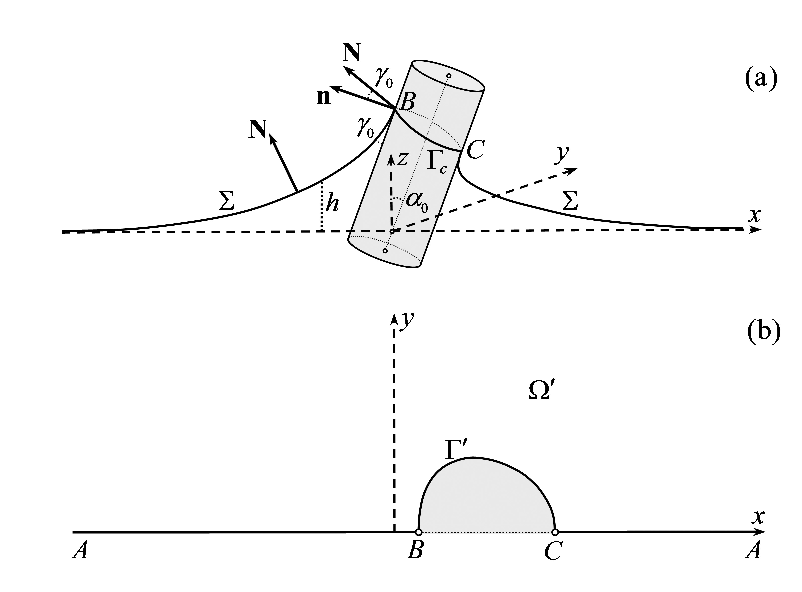
\includegraphics[clip,width=95mm]{Alimov_Fig1.eps}
 \caption {(a) Schematic representation of the external meniscus $\Sigma$ on an inclined fiber with circular
cross-section. (b) Projection of the symmetry element of $\Sigma$ in half-space $y \ge 0$ onto the
$xy$-plane. Vector ${\rm {\bf N}} = \left( {N_x, N_y, N_z} \right)$ denotes the normal to the
meniscus $\Sigma$. Vector ${\rm {\bf n}} = \left( {n_x, n_y, n_z}\right)$ denotes the normal to the
lateral surface of the fiber.}
 \label{Alimov_Fig1}
\end{figure}

Using function $h(x,y)$, we can find an analytical expression for the normal ${\rm {\bf N}}$ to the
meniscus $\Sigma$~\cite{Alimov:bib11}
\begin{equation}
\label{Alimov:eq2} {\rm {\bf N}} = \left( {1\hspace{-0.5mm}+\hspace{-0.5mm}\vert \nabla h\vert^2}
\right)^{-1 \left/ 2 \right.} \left( {- \frac{\partial h}{\partial x}, - \frac{\partial h}{\partial
y}, 1} \right).
\end{equation}
Then, the mathematical model of the capillary rise of the liquid on the inclined fiber can be formally
written in a form similar to that of the vertical fiber~\cite{Alimov:bib5}
\begin{equation}
\label{Alimov:eq3} {\Omega }':\quad \nabla \cdot \left[ {\left(
1\hspace{-0.5mm}+\hspace{-0.5mm}\vert \nabla h \vert^{2} \right)^{-1/2} \nabla h } \right] -
\varepsilon h = 0,
\end{equation}
\begin{equation}
\label{Alimov:eq4} {\Gamma }':\quad {\rm {\bf N}} \cdot {\rm {\bf n}} = \cos \gamma _0,
\end{equation}
\begin{equation}
\label{Alimov:eq5} AB \cup CA:\quad {\partial h} \left/{\partial y} \right. = 0,
\end{equation}
\begin{equation}
\label{Alimov:eq6} r = \sqrt {x^2 + y^2} \to \infty : \quad h(x,y) \to 0.
\end{equation}

Here the first term of equation~\eqref{Alimov:eq3} represents the average curvature of the meniscus
$\Sigma$~\cite{Alimov:bib11}, the second term is the hydrostatic pressure, and the equation as a
whole is Laplace's capillary law~\cite{Alimov:bib12}. Vector ${\rm {\bf n}} = \left( {n_x, n_y, n_z
} \right)$ denotes the normal to the lateral surface of the fiber. The boundary
condition~\eqref{Alimov:eq4} is the Young-Laplace condition of dynamic equilibrium of the contact
line $\Gamma_c $~\cite{Alimov:bib1}. The boundary condition~\eqref{Alimov:eq5} is the condition of
smooth symmetrical continuation of the meniscus $\Sigma$ across the boundaries $AB$ and $CA$, see
Fig.~\ref{Alimov_Fig1}~a. If the fiber cross-section is given, then the boundary value
problem~\eqref{Alimov:eq3}--\eqref{Alimov:eq6} depends on the two physical parameters, namely on
the contact angle $\gamma_0$ and on the angle of fiber inclination $\alpha_0$.

Let us emphasize two features of this problem that significantly complicate its analysis in
comparison with the case of the vertical fiber:

\textbf{(i)} Even in the simplest case of the inclined fiber with the circular cross-section, the
condition~\eqref{Alimov:eq4} is written on the contour ${\Gamma}'$ of unknown shape. The shape of
${\Gamma}'$ must also be determined.

\textbf{(ii)} The use of the function~\eqref{Alimov:eq1} is possible only under the restriction
$\gamma_0 \ge \alpha_0$ since its violation leads to loss of one-valuedness for the
function~\eqref{Alimov:eq1} in the vicinity of the point $C$, see Fig.~\ref{Alimov_Fig1}a. At the
same time the all physical assumptions concerning the
problem~\eqref{Alimov:eq3}--\eqref{Alimov:eq6} remain valid.

\section{Asymptotic approach for thin fibers} \label{Alimov:sec2}
Let the fiber be thin, i.e., $L_m \ll L_c$. Then, the Bond number becomes small, $\varepsilon \ll 1$,
and asymptotic methods can be used. The well-known asymptotic approach for the case of the vertical
thin fiber~\cite{Alimov:bib5} allows a formal generalization to the case of the inclined thin
fiber; but such a simple formal generalization is ineffective, since both indicated features
\textbf{(i)} and \textbf{(ii)} of problem~\eqref{Alimov:eq3}--\eqref{Alimov:eq6} are preserved for
small $\varepsilon \ll 1$, see~\cite{Alimov:bib9}. For example, even the simplest case of the
inclined thin fiber with the circular cross-section cannot be analyzed. At the same time, in the
article~\cite{Alimov:bib9} it was shown that the approach~\cite{Alimov:bib5} can be supplemented by
a transformation to the new Cartesian coordinate system that is associated with the inclined fiber.
This allows eliminating both indicated features \textbf{(i)} and \textbf{(ii)} of the
problem~\eqref{Alimov:eq3}--\eqref{Alimov:eq6}.

Now, following~\cite{Alimov:bib9}, we introduce a new Cartesian coordinate system $XYZ$, which is
obtained by rotating the coordinate system $xyz$ around the axis $y$ by the angle of $\alpha_0$,
see Fig.~\ref{Alimov_Fig2}~a. Then, the axis $Z$ coincides with the central axis of the fiber and the
plane $XY$ is strictly perpendicular to the fiber axis. Obviously, we have identity
\begin{equation}
\label{Alimov:eq7} Y = y,
\end{equation}
 and, therefore, we are dealing with a simpler transformation $xz \to XZ$ of the Cartesian
coordinate system $xz$ by rotating it relative to the origin by the angle $( - \alpha_0 ) < 0$.
Here we use the generally accepted rule in analytical geometry for choosing positive directions of
angles~\cite{Alimov:bib13}.

Let us present the resulting formulas for both the direct transformation of coordinates $xz \to XZ$
and the inverse transformation of coordinates $XZ \to xz$~\cite{Alimov:bib13}
\begin{equation}
\label{Alimov:eq8}
 \left\{ {{\begin{array}{l}
 X = x\cos \alpha_0 - z\sin \alpha_0, \hfill \\
 Z = x\sin \alpha_0 + z\cos\alpha_0, \hfill \\
\end{array} }} \right.
\quad\quad \Leftrightarrow \quad\quad
 \left\{ {{\begin{array}{l}
 x = X\cos \alpha_0 + Z\sin \alpha_0, \hfill \\
 z = - X\sin \alpha_0 + Z\cos \alpha_0. \hfill \\
\end{array} }} \right.
\end{equation}
\begin{figure}%[!tbh]
\renewcommand{\figurename}{Fig.} \centering
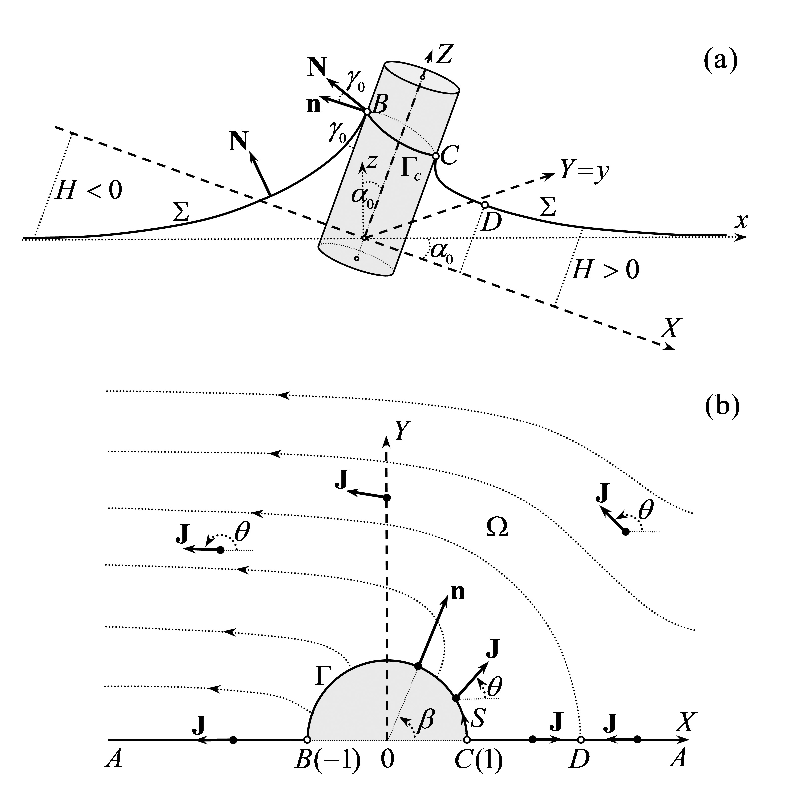
\includegraphics[clip,width=90mm]{Alimov_Fig2.eps}
\caption{(a) Schematic representation of the external meniscus $\Sigma$ in the Cartesian coordinate
system $XYZ$ associated with the fiber. (b) Projection of the symmetry element of $\Sigma$ in
half-space $Y \ge 0$ onto the $XY$-plane; the dashed lines show the streamline pattern for the
fictitious flow ${\rm {\bf J}}$.}
 \label{Alimov_Fig2}
\end{figure}

Now we can make the transition from the definition of the surface $\Sigma $ by using the function
$h(x,y)$ in space $(x, y, z)$, see~\eqref{Alimov:eq1}, to the definition of the same surface by
using a function $H(X,Y)$ in space $(X, Y, Z)$
\begin{equation}
\label{Alimov:eq9} \Omega :\quad Z = H(X,Y),
\end{equation}
where $\Omega$ is a region obtained by the projection of the symmetry element of the
surface $\Sigma$ in the half-space $Y > 0$ on the plane $XY$, see Fig.~\ref{Alimov_Fig2}~b; the
value of $H(X,Y)$ is the $Z$-coordinate of the meniscus $\Sigma$ at the point $(X,Y) \in \Omega$,
see Fig.~\ref{Alimov_Fig2}~a. We note that, in contrast to the region ${\Omega}'$, $\Omega$ is the
region of known shape. Indeed, it is clear from Fig.~\ref{Alimov_Fig2}~b that region $\Omega$ is the
upper half of the exterior of the contour $\Gamma$ (unit circle). Note also that the
function~\eqref{Alimov:eq9} can be used for any combination of the angles $\gamma_0 $ and $\alpha_0
$, since $H(X,Y)$ always remains the one-valued function for typical configurations of the meniscus
$\Sigma$, see Fig.~\ref{Alimov_Fig2}~b. Thus, having made the transition from the function $h(x,y)$
to the function $H(X,Y)$, we got rid of both indicated features \textbf{(i)} and \textbf{(ii)} of
the problem~\eqref{Alimov:eq3}--\eqref{Alimov:eq6}.

Taking into account the formula~\eqref{Alimov:eq8}, we can establish a relation between the
functions $h(x,y)$ and $H(X,Y)$
\[
 h(x,y) = - X\sin \alpha_0 + H(X,Y)\cos \alpha_0 .
\]
In particular, it follows from this relation that there are two equivalent records for an equation
of a horizontal plane as some approximate equation of the meniscus $\Sigma$ at infinity
\begin{equation}
\label{Alimov:eq10} r \to \infty :\quad z \approx 0\quad \quad \Leftrightarrow \quad \quad R \to
\infty :\quad Z \approx X\tan \alpha_0,
\end{equation}
where $r = \sqrt {x^2 + y^2} $ and $R = \sqrt {X^2 + Y^2} $.

The normal ${\rm {\bf N}}$ to the meniscus $\Sigma$ can be expressed in terms of the function
$H(X,Y)$ by analogy with~\eqref{Alimov:eq2}
\begin{equation}
\label{Alimov:eq11} {\rm {\bf N}} = \left( {1\hspace{-0.5mm}+\hspace{-0.5mm}\vert \nabla
H(X,Y)\vert^{2}} \right)^{-1/2}\left( { - \frac{\partial H}{\partial X}, - \frac{\partial
H}{\partial Y}, 1} \right).
\end{equation}
Then, the problem~\eqref{Alimov:eq3}--\eqref{Alimov:eq6} can be rewritten in terms of the function
$H(X,Y)$, next the assumption $\varepsilon \ll 1$ can be accepted, and the method of asymptotic
matching can be applied to this rewritten problem. This was done in the paper~\cite{Alimov:bib9}.
As a result, it was shown that the outer asymptotic expansion $H \approx H^{(o)}(X,Y)$ approximates
the meniscus $\Sigma$ in the zone $R \sim \varepsilon ^{-1 \left/ 2 \right.}$. The leading term of
this expansion has the form~\cite{Alimov:bib9}
\begin{equation}
\label{Alimov:eq12} H^{(o)}\hspace{-0.5mm}\left( {X,Y} \right) = X\tan \alpha_0 + \frac{Q}{2\pi
\cos \alpha_0} K_0\hspace{-1mm}\left({\varepsilon^{1/2}\sqrt{\frac{X^2}{\cos ^2\alpha_0
}+Y^2}}\right),
\end{equation}
 where $K_0$ is the Bessel function of the second kind~\cite{Alimov:bib14} and $Q$ is an
parameter of the asymptotic matching (an undetermined real constant).

The inner asymptotic expansion $H \approx H^{(i)}(X,Y)$ approximates the meniscus $\Sigma $ in the
fiber neighborhood $R \sim 1$. The leading term of this expansion satisfies the boundary value
problem~\cite{Alimov:bib9}
\begin{equation}
\label{Alimov:eq13} \Omega :\quad \nabla \cdot \left[ {\left(
1\hspace{-0.5mm}+\hspace{-0.5mm}\vert\nabla H^{(i)}\vert^{2} \right)^{- 1/2}\nabla H^{(i)}} \right]
= 0,
\end{equation}
\begin{equation}
\label{Alimov:eq14} \Gamma :\quad -\left( 1\hspace{-0.5mm}+\hspace{-0.5mm}\vert\nabla
H^{(i)}\vert^{2} \right)^{-1/2}\nabla H^{(i)} \cdot {\rm {\bf n}} = \cos \gamma_0,
\end{equation}
\begin{equation}
\label{Alimov:eq15} AB \cup CA:\quad {\partial H^{(i)}}\hspace{-0.5mm}/{\partial Y} = 0,
\end{equation}
\begin{equation}
\label{Alimov:eq16} R \gg 1:\quad  H^{(i)}(X,Y) = X \tan \alpha_0 - \frac{Q}{2\pi \cos \alpha_0}
\left[ {\ln \sqrt {\frac{X^2}{\cos^2\alpha_0 } + Y^2}+C_\varepsilon } \right] + O\left( {R^{-1}\ln
R} \right).
\end{equation}
Here we denote as $C_\varepsilon$ such constant
\begin{equation}
\label{Alimov:eq17} C_\varepsilon = \ln \left( {0.5 \varepsilon^{1/2} e^E} \right),
\end{equation}
where $E = 0.57...$ is the Euler constant~\cite{Alimov:bib14}.

The governing differential equation~\eqref{Alimov:eq13} is essentially the minimal surface
equation, as in the case of the vertical thin fiber~\cite{Alimov:bib5}. The condition at
infinity~\eqref{Alimov:eq16} is the result of matching with the main term of the outer asymptotic
expansion~\eqref{Alimov:eq12}. The Young--Laplace condition~\eqref{Alimov:eq14} essentially
coincides with the condition~\eqref{Alimov:eq4}. The vector ${\rm {\bf n}}$ also denotes the normal
to the fiber surface. However, in the new coordinate system $XYZ$ the $Z$-component of this normal
is equal to zero. If we introduce the notation $\beta$ for the inclination angle of the normal
${\rm {\bf n}}$ to the $X$-axis, then we get an analytical expression: ${\rm {\bf n}} = (\cos
\beta, \sin \beta, 0)$ (see Fig.~\ref{Alimov_Fig2}b).

Suppose that the solution of the problem~\eqref{Alimov:eq13}--\eqref{Alimov:eq16} has been found,
i.e., that the leading term of the inner asymptotic expansion $H^{(i)}(X,Y)$ is known. Then, using
the procedure of the asymptotic matching~\cite{Alimov:bib15}, we can find the leading term of the
asymptotic expansion $H^{(u)}(X,Y)$, which uniformly approximates the meniscus $\Sigma$ everywhere
in the $XY$-plane~\cite{Alimov:bib9}
\begin{equation}
\label{Alimov:eq18} H^{(u)}(X,Y)\hspace{-0.5mm} =\hspace{-0.5mm}
H^{(i)}(X,Y)\hspace{-0.5mm}+\hspace{-0.5mm}\frac{Q}{2\pi \cos \alpha_0 }\left[ {K_0\hspace{-1mm}
\left( {\varepsilon^{1/2} \sqrt {\frac{X^2}{\cos^2\alpha_0 }\hspace{-0.5mm}+\hspace{-0.5mm}Y^2} }
\right)\hspace{-1mm}+\hspace{-0.5mm}\ln \sqrt {\frac{X^2}{\cos^2\alpha_0
}\hspace{-0.5mm}+\hspace{-0.5mm}Y^2}+C_\varepsilon } \right]\hspace{-0.5mm}.
\end{equation}

In addition, the parameter $Q$ can be found in advance, even before solving the
problem~\eqref{Alimov:eq13}--\eqref{Alimov:eq16}, by using the formula~\cite{Alimov:bib9}
\begin{equation}
\label{Alimov:eq19} Q = \frac{l\cos \gamma_0 }{\cos \alpha_0 } = \frac{2\pi \cos \gamma_0 }{\cos
\alpha_0 },
\end{equation}
since we know a priori the perimeter $l$ of the fiber cross-section $\Gamma$ (unit
circle): $l = 2\pi$.

It only remains to find the solution $H^{(i)}(X,Y)$ to the problem of the internal asymptotic
expansion~\eqref{Alimov:eq13}--\eqref{Alimov:eq16}. Note that the behavior of the function
$H^{(i)}(X,Y)$ at infinity in this problem differs from the case of the vertical thin
fiber~\cite{Alimov:bib5}. In addition to the logarithmic singularity, here we have a higher order
singularity, namely the linear term $X \tan \alpha_0 $, see the condition~\eqref{Alimov:eq16}. The
structure of the logarithmic term itself is also slightly different from~\cite{Alimov:bib5}.
Nevertheless, we can hope that some solutions of the
problem~\eqref{Alimov:eq13}--\eqref{Alimov:eq16} can be constructed if we apply the same
mathematical apparatus that was effectively applied in the case of the vertical thin fiber. This
apparatus includes an analogy with the theory of flows of non-Newtonian fluids through porous
media~\cite{Alimov:bib16} and the Chaplygin's hodograph transformation~\cite{Alimov:bib17}.

\section{Analogy with flows of non-Newtonian fluids through porous media. Chaplygin's hodograph
transformation.} \label{Alimov:sec3}
 Let us define a fictitious flow of incompressible fluid
through a porous medium ${\rm {\bf J}}$ such that
\begin{equation}
\label{Alimov:eq20} \Omega :\quad {\rm {\bf J}} = - \frac{\nabla H^{(i)}}{\sqrt
{1\hspace{-0.5mm}+\hspace{-0.5mm} \vert \nabla H^{(i)}\vert^2} },\quad \nabla \cdot {\rm {\bf J}}=0,
\end{equation}
where the function $H^{(i)}(X,Y)$ is an analogue of the pressure in the
liquid~\cite{Alimov:bib16}. Here the first relation represents the nonlinear law of flow of
non-Newtonian fluid in porous media, the second relation is the continuity equation, and the
formula~\eqref{Alimov:eq20}) as a whole represents another form of writing for the
equation~\eqref{Alimov:eq13}.

The fictitious flow ${\rm {\bf J}}$ is characterized by its magnitude $J$ and by its inclination
angle $\theta$ to the $X$-axis, i.e. ${\rm {\bf J}} = J\left( {\cos \theta, \sin \theta} \right)$.
If we compare the formulas~\eqref{Alimov:eq20} and~\eqref{Alimov:eq11}, we come to the conclusion
that the fictitious flow ${\rm {\bf J}}$ is equal to the projection of the normal ${\rm {\bf N}}$
onto the $XY$-plane. Since we have some general representation of the shape of the meniscus
$\Sigma$, we can imagine the behavior of the vector field ${\rm {\bf J}}(X,Y)$ in region $\Omega$.
As a result, we can imagine the streamline pattern that corresponds to the fictitious flow ${\rm
{\bf J}}$, see dotted lines in Fig.~\ref{Alimov_Fig2}~b. In particular, it is easy to establish that
at some point $D \in CA$ the tangent to the meniscus $\Sigma$ is strictly parallel to the
$XY$-plane. Accordingly, for the vector field ${\rm {\bf J}}(X,Y)$ of the fictitious flow, the
point $D$ is the flow stagnation point for which $J = 0$.

Since the fluid is incompressible, we can introduce a stream function $\psi
(X,Y)$~\cite{Alimov:bib18}. Using the formula~\eqref{Alimov:eq20}, we obtain
\[
J = \vert \nabla H^{(i)}\vert \left( {1\hspace{-0.5mm}+\hspace{-0.5mm}\vert \nabla H^{(i)}\vert^2}
\right)^{-1/2}\quad \Leftrightarrow \quad \vert \nabla H^{(i)}\vert = J\left( {1-J^2}
\right)^{-1/2}.
\]
This one-to-one correspondence between the values $J$ and $\vert \nabla H^{(i)}\vert $ allows us to
use of the Chaplygin's hodograph transformation~\cite{Alimov:bib17}. All the mathematical details
of the application of this transformation to the problems of capillary rise of liquid along thin
fibers have already been published many times, see~\cite{Alimov:bib5}--\cite{Alimov:bib8}.
Therefore, here we present only a summary of the main formulas for applying the Chaplygin's
hodograph transformation to the problem~\eqref{Alimov:eq13}--\eqref{Alimov:eq16}:
\begin{equation}
\label{Alimov:eq21} J_X = J\cos \theta = \frac{\partial \psi}{\partial Y},\quad J_Y = J\sin \theta
=-\frac{\partial \psi}{\partial X},
\end{equation}
\[
\nabla H^{(i)}(X,Y) = -\left( {1-J^2} \right)^{-1/2}{\rm {\bf J}},
\]
\begin{equation}
\label{Alimov:eq22} J = \frac{1}{\cosh t} \quad  \Leftrightarrow \quad t = \mbox{arccosh}\,
\frac{1}{J},
\end{equation}
\[
0 \le \vert \nabla H^{(i)}(X,Y)\vert \le \infty ,\quad 0\le J\le 1,\quad 0\le t \le \infty,
\]
\begin{equation}
\label{Alimov:eq23} \frac{\partial \psi}{\partial t} = \frac{\partial H^{(i)}}{\partial \theta},
\quad \frac{\partial \psi}{\partial\theta } = -\frac{\partial H^{(i)}}{\partial t}.
\end{equation}

As a result of applying the Chaplygin's transformation, we arrive at the Cauchy--Riemann
equations~\eqref{Alimov:eq23}, which allows us to introduce complex variables $W$ and $\chi$
\[
W = - H^{(i)} + i \psi,\quad \quad \chi = t + i\theta,
\]
where $W$ is called the complex velocity potential, and $\chi $ is called the hodograph
(these are conventional names, see~\cite{Alimov:bib16}). Accordingly, we can use two functions of
the complex variables, namely $W(\chi)$ and $\chi(W)$~\cite{Alimov:bib19}.

If one of these functions is found, we can then return to the variables $X$ and $Y$ by writing
Khristianovich's formulas for the total differentials of functions $X(H^{(i)}\hspace{-0.5mm},\psi)$
and $Y(H^{(i)}\hspace{-0.5mm},\psi)$~\cite{Alimov:bib16}
\begin{equation}
\label{Alimov:eq24} dX = - \cos \theta \sinh t\,dH^{(i)} - \sin \theta \cosh t\,d\psi ,\quad dY =
-\sin \theta \sinh t\,dH^{(i)} + \cos \theta \cosh t\,d\psi .
\end{equation}

In order to find one of the functions $W(\chi)$ or $\chi(W)$, let us rewrite the boundary value
problem~\eqref{Alimov:eq13}--\eqref{Alimov:eq16} in terms of complex variables $\chi$ and $W$.
Consider the differential equation~\eqref{Alimov:eq13}. As shown above, a consequence of this
equation is the fact that $W(\chi)$ and $\chi(W)$ are functions of complex variable.

Consider now the condition~\eqref{Alimov:eq14} at the boundary $\Gamma$. First, we write it in
terms of the fictitious flow ${\rm {\bf J}}$, using the formula~\eqref{Alimov:eq20}
\begin{equation}
\label{Alimov:eq25} \Gamma : \quad {\rm {\bf J}} \cdot {\rm {\bf n}} = \cos \gamma_0.
\end{equation}
The scalar product on the left-hand side of~\eqref{Alimov:eq25} can be expressed through the
difference between the angles $\theta$ and $\beta$: ${\rm {\bf J}} \cdot {\rm {\bf n}} = J\cos
(\theta - \beta)$, see Fig.~\ref{Alimov_Fig2}~b. Then, using the relationship~\eqref{Alimov:eq22}
between the values $J$ and $t$, the condition~\eqref{Alimov:eq25} can be rewritten in terms of the
hodograph $\chi$
\begin{equation}
\label{Alimov:eq26} \Gamma :\quad \cos (\theta - \beta ) = \cos \gamma_0 \cosh t.
\end{equation}

Note that this condition in the form~\eqref{Alimov:eq25} allows us to accurately determine the
amount of fictitious fluid $M$ entering per unit time the region $\Omega$ through the boundary
$\Gamma$
\begin{equation}
\label{Alimov:eq27} M = \pi \cos \gamma_0.
\end{equation}

Accordingly, the amount of fictitious fluid entering through the full cross section of the fiber is
equal to $2M$. The fictitious fluid is incompressible, and the two remaining boundaries of the
region $\Omega$, namely $AB$ and $CA$, are impermeable. Therefore, there must be a singularity at
infinity, namely sink of the same strength $2M = 2\pi \cos \gamma_0 $. In addition, according to
both the condition~\eqref{Alimov:eq16} and the streamline pattern for the fictitious flow ${\rm
{\bf J}}$ in Fig.~\ref{Alimov_Fig2}~b, there must be another singularity at infinity, namely the
dipole singularity~\cite{Alimov:bib18}.

The condition~\eqref{Alimov:eq15} can easily be rewritten in terms of $W$ and $\chi$ if we take
into account the same streamline pattern in Fig.~\ref{Alimov_Fig2}~b and the value of $M$,
see~\eqref{Alimov:eq27}
\begin{equation}
\label{Alimov:eq28} CD \cup DA: \quad \psi = 0; \quad \quad AB:\quad \psi = \pi \cos \gamma_0,
\end{equation}
\begin{equation}
\label{Alimov:eq29} CD:\quad \theta = 0; \quad \quad DA \cup AB:\quad \theta = \pi.
\end{equation}

Finally, consider the condition~\eqref{Alimov:eq16} at infinity. The infinity $A \in DA$
corresponds to $X \to + \infty$ and the infinity $A \in AB$ corresponds to $X \to - \infty $, see
Fig.~\ref{Alimov_Fig2}b. It is clear that it is the first term in this condition that determines
the behavior of the function $H^{(i)}(X,Y)$ at infinity. Taking into account the
condition~\eqref{Alimov:eq28}, we obtain directly from the condition~\eqref{Alimov:eq16}
\begin{equation}
\label{Alimov:eq30} A \in DA: \quad  H^{(i)} \to + \infty,\quad \psi = 0;\quad \quad A \in AB:\quad
H^{(i)} \to - \infty,\quad \psi = \pi \cos \gamma_0 .
\end{equation}
The formula~\eqref{Alimov:eq30} expresses the condition at infinity~\eqref{Alimov:eq16} in terms of
the complex velocity potential $W$. In order to find this condition in terms of the hodograph
$\chi$, it is necessary to obtain estimates of the fictitious flow ${\rm {\bf J}}$ at infinity.

Let us introduce the following notation
\[
{\rm {\bf E}}_0 = \left( {1, 0} \right),\quad \quad {\rm {\bf R}} = \left( {X,\;Y} \right), \quad
\quad {\rm {\bf R}}_{\rm {\bf 1}} = \left( {X\cos^{-2}\alpha_0, Y} \right).
\]
Then, by differentiating the equation~\eqref{Alimov:eq16}, we obtain the relation
\[
R \gg 1:\quad \quad \nabla H^{(i)}(X,Y) = \tan \alpha_0 \,{\rm {\bf E}}_{\rm {\bf 0}} - \left(
{\frac{Q}{2\pi \cos \alpha_0 }} \right)\frac{{\rm {\bf R}}_{\rm {\bf 1}} } {X^2\cos^{-2}\alpha_0 +
Y^2} + o\left( R^{-1} \right).
\]
Substituting this relation into the first expression of~\eqref{Alimov:eq20}, we obtain the estimate
of the fictitious flow ${\rm {\bf J}}$ at infinity (see~\cite{Alimov:bib9} for details)
\[
R \gg 1: \quad {\rm {\bf J}} = - \sin \alpha_0 \,{\rm {\bf E}}_{\rm {\bf 0}} + \left(
{\frac{Q}{2\pi}} \right)\frac{{\rm {\bf R}}}{X^2\cos^{-2}\alpha_0 + Y^2} + o\left( {R^{-1}}
\right).
\]
Using this, we can estimate the leading term of the asymptotic expansion of ${\rm {\bf J}}$ in
powers of $R^{-1}$ as ${\rm {\bf J}} \approx - \sin \alpha_0 {\rm {\bf E}}_0$. As a result, the
condition at infinity~\eqref{Alimov:eq16} in terms of the hodograph $\chi$ takes the form
\begin{equation}
\label{Alimov:eq31} A: \quad J_A = \sin \alpha_0, \quad t_A = \mbox{arccosh}\, \left(
{\frac{1}{\sin \alpha_0 }} \right) = \ln \left( {\frac{1 + \cos \alpha_0 }{\sin \alpha_0}} \right),
\quad \theta_A = \pi,
\end{equation}
where the formulas~\eqref{Alimov:eq22} and~\eqref{Alimov:eq29} were also taken into
account.

\section{The particular case of full wetting. The $\chi$- and $W$-planes} \label{Alimov:sec4}
Examples of determining the configuration of external menisci on vertical thin
fibers~\cite{Alimov:bib5},~\cite{Alimov:bib6},~\cite{Alimov:bib8} showed that the use of the
Chaplygin's transformation is most effective in the particular case of full wetting of the fiber.
We also limit ourselves to this particular case, i.e., we accept $\gamma_0 = 0$ here and in the
sequel. Then, using the formula~\eqref{Alimov:eq19}, we can immediately find the value of $Q$:
\begin{equation}
\label{Alimov:eq32} Q = \frac{2\pi}{\cos \alpha_0 }.
\end{equation}

It can easily be checked that in the particular case $\gamma_0 = 0$ the boundary
conditions~\eqref{Alimov:eq28}--\eqref{Alimov:eq30} take the form
\begin{equation}
\label{Alimov:eq33} CD \cup DA: \quad \psi = 0; \quad \quad AB: \quad \psi = \pi,
\end{equation}
\begin{equation}
\label{Alimov:eq34} CD:\quad \theta = 0; \quad \quad DA \cup AB: \quad \theta = \pi ,
\end{equation}
\begin{equation}
\label{Alimov:eq35} A \in DA: \quad H^{(i)} \to +\infty, \quad \psi = 0; \quad \quad A \in AB:
\quad H^{(i)} \to -\infty, \quad \psi = \pi,
\end{equation}
we must add to this system of equations the condition~\eqref{Alimov:eq31}, the form of
which does not change.

Let us try to determine the shape of the regions $\Omega_\chi $ and $\Omega_W $ corresponding to
the region $\Omega$ in the $\chi$- and $W$-planes. For this purpose we use the boundary conditions
in terms $\chi$ and $W$, which have been obtained in Section 3.

In the case of full wetting, at every point of the contact line $\Gamma_c $ the normal to the
meniscus ${\rm {\bf N}}$ obviously coincides with the normal to the fiber ${\rm {\bf n}}$, see
Fig.~\ref{Alimov_Fig2}~a. This implies that $\vert \nabla H \vert \to \infty $ and the normal ${\rm
{\bf N}}$ is parallel to the $XY$-plane. Then, the equality
\[
\Gamma _c: \quad {\rm {\bf J}} = {\rm {\bf N}} = {\rm {\bf n}}
\]
is satisfied on the contact line $\Gamma_c $. As a result, the different
forms~\eqref{Alimov:eq14},~\eqref{Alimov:eq25}, and~\eqref{Alimov:eq26} of the condition at the
boundary $\Gamma$ gives
\begin{equation}
\label{Alimov:eq36} \Gamma: \quad \theta = \beta, \quad J \equiv J_n = 1, \quad t = 0.
\end{equation}

At the point $D$ of the boundary $CA$ we have: normal ${\rm {\bf N}}$ is perpendicular to the
$XY$-plane, $J = 0$ and, therefore, $t \to +\infty $. Taking into account this fact together with
the conditions~\eqref{Alimov:eq31},~\eqref{Alimov:eq34}, and~\eqref{Alimov:eq36}, we conclude that
the region $\Omega_\chi $ in the complex plane of hodograph $\chi = t + i\theta$ is the half-strip,
shown in Fig.~\ref{Alimov_Fig3}~a.
\begin{figure}%[!tbh]
\renewcommand{\figurename}{Fig.} \centering
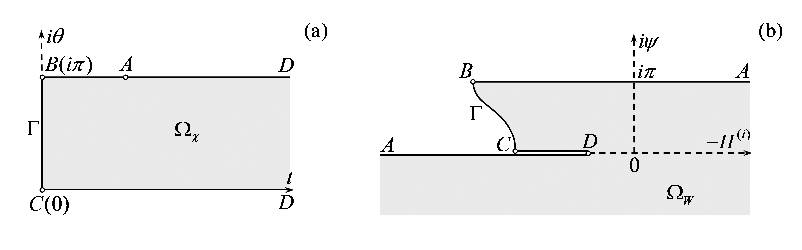
\includegraphics[clip,width=130mm]{Alimov_Fig3.eps}
\caption{(a) Plane of the hodograph $\chi = t + i\theta$. (b) Plane of the complex velocity
potential $W = -H^{(i)} + i\psi $. In the $W$-plane, the shape of the boundary $\Gamma$ is unknown.}
 \label{Alimov_Fig3}
\end{figure}

In order to find the shape of the region $\Omega_W$ in the plane of the complex velocity potential
$W = - H^{(i)} + i\psi$, we use the boundary conditions~\eqref{Alimov:eq33}
and~\eqref{Alimov:eq35}. Then, we get the region shown in Fig.~\ref{Alimov_Fig3}~b. It should be
note the important feature of all
forms~\eqref{Alimov:eq14},~\eqref{Alimov:eq25},~\eqref{Alimov:eq26}, and~\eqref{Alimov:eq36} of the
condition at the boundary $\Gamma$: they contain no information whatever about the behavior of
$H^{(i)}$ or $\psi$. Therefore, $\Gamma$ is the boundary of unknown shape in the $W$-plane, and
Fig.~\ref{Alimov_Fig3}~b shows only the hypothetical shape of this boundary. As a result, we
cannot solve the problem of determining the function $W(\chi)$ by using the method of conformal
mapping~\cite{Alimov:bib19}.

\subsection{Transition to the derivative ${dW}/{d\chi}$} \label{Alimov:subsec5.1}
We propose to introduce an auxiliary function $F(\chi )$, which is obtained by differentiating
$W(\chi)$
\begin{equation}
\label{Alimov:eq37} F(\chi) = \frac{dW}{d\chi}.
\end{equation}

Let us investigate the boundary behavior of this function. In order to estimate its behavior on the
boundary $\Gamma$, we introduce the arc length $S$, which is measured along the contour $\Gamma \in
XY$ from the point $C$, see Fig.~\ref{Alimov_Fig2}~b. Taking into account the
property~\eqref{Alimov:eq21} of the stream function $\psi$, we can write the boundary relation on
this contour
\begin{equation}
\label{Alimov:eq38} \Gamma :\quad \frac{d\psi}{dS} = J_n.
\end{equation}

The contour $\Gamma \in XY$ is the unit circle. Then, taking into account
formulas~\eqref{Alimov:eq36} and~\eqref{Alimov:eq38}, we obtain an important identity for some
differentials along this contour
\begin{equation}
\label{Alimov:eq39} \Gamma :\quad d\psi = dS = d\theta = d\beta.
\end{equation}

Note that the variable $t$ at the boundary $\Gamma$ in the $\chi$-plane remains constant, see
Fig.~\ref{Alimov_Fig3}~a. Therefore, we can write the derivative ${dW}/d{\chi}$ at this boundary in
the form~\cite{Alimov:bib19}
\begin{equation}
\label{Alimov:eq40} \Gamma :\quad \frac{dW}{d\chi} = \frac{1}{i}\frac{d}{d\theta}\left( {-H^{(i)}+
i\psi} \right) = \frac{d\psi}{d\theta}+i\frac{dH^{(i)}}{d\theta}.
\end{equation}
As a result, using formulas~\eqref{Alimov:eq39} and~\eqref{Alimov:eq40}, we find the behavior of
the function $F = {dW}/{d\chi}$ at this boundary
\begin{equation}
\label{Alimov:eq41} \Gamma :\quad \mbox{Re}\, F = 1.
\end{equation}

Next, we estimate the behavior of the function $F(\chi )$ on the remaining boundaries $AB$, $DA$, and
$CD$. Note that the variable $\theta$ at each of these boundaries remains constant, see
Fig.~\ref{Alimov_Fig3}~a. Similar to~\eqref{Alimov:eq40}, we can express the derivative
${dW}/{d\chi}$ at these boundaries in the form~\cite{Alimov:bib19}
\begin{equation}
\label{Alimov:eq42} AB \cup DA \cup CD: \quad \frac{dW}{d\chi } = \frac{d}{dt}\left( {-H^{(i)} +
i\psi } \right) = - \frac{dH^{(i)}}{dt} + i\frac{d\psi}{dt}.
\end{equation}
As a result, using formulas~\eqref{Alimov:eq33} and~\eqref{Alimov:eq42}, we find the behavior of
the function $F = {dW}/{d\chi}$ at these boundaries
\begin{equation}
\label{Alimov:eq43} AB \cup CD \cup DA: \quad \mbox{Im} \, F = 0.
\end{equation}

We should add to this condition the inequality
\begin{equation}
\label{Alimov:eq44} AB \cup CD \cup DA: \quad \mbox{Re} \,F = - \frac{dH^{(i)}}{dt} \ge 0,
\end{equation}
which is obtained from formula~\eqref{Alimov:eq42} by taking into account the known
behavior of the variables $H^{(i)}$ and $t$ at the boundaries $AB \cup DA \cup CD$ in the
$\chi$-plane and in the $W$-plane, see Fig.~\ref{Alimov_Fig3}.

Further, by comparing Fig.~\ref{Alimov_Fig3}~a with Fig.~\ref{Alimov_Fig3}b it is easily established
that at the points $A$ and $D$ the conformality property of the mapping $\chi \to W$ is violated.
Then the modulus $\vert F\vert = \vert {dW}/{d\chi}\vert$ at these points is equal to zero or
infinity~\cite{Alimov:bib19}. In the $W$-plane, we have $\vert W\vert \to \infty $ at point $A$, and,
therefore, in the $F$-plane we get~\cite{Alimov:bib19}
\begin{equation}
\label{Alimov:eq45} A:\quad \vert F \vert \to \infty .
\end{equation}

Let us turn to the point $D$. According to Figs.~\ref{Alimov_Fig3}~a and b, for
the conformal mapping $\chi \to W$ in the neighborhood of this point, the following estimates
hold~\cite{Alimov:bib19}
\[
W \sim W_D: \quad \chi (W) \sim -\frac{1}{2}\ln \left( {W_D - W} \right); \quad \Rightarrow \quad
W(\chi) \sim W_D - e^{-2\chi}; \quad \Rightarrow \quad \frac{dW}{d\chi} \sim 2e^{-2t- 2i\theta}.
\]
At the point $D$ of the $\chi$-plane we have $t \to +\infty $, see Fig.~\ref{Alimov_Fig3}~a. As a
result, the function $F = {dW}/{d\chi}$ at this point can be evaluated explicitly
\begin{equation}
\label{Alimov:eq46} D: \quad F = 0.
\end{equation}
Using~\eqref{Alimov:eq41} and~\eqref{Alimov:eq43}--\eqref{Alimov:eq46}, we can estimate the
boundary behavior of the function $F(\chi)$. As a result, we conclude that the region $\Omega_F$ in
the plane of complex variable $F$ is the plane with a polygonal cut, as shown in
Fig.~\ref{Alimov_Fig4}~a. Regions of this type in the theory of functions of a complex variable are
called star-like regions [19]. Note that we additionally introduce the auxiliary point $E$ in
Fig.~\ref{Alimov_Fig4}a, so that the value $F = 1$ in the region $\Omega_F $ now corresponds to
three boundary points $B$, $C,$ and $E$, each of which lie on different banks of the polygonal cut.
We should also note that the length of segment $BC = \Gamma$ in the $F$-plane is not known in
advance.
Thus, the regions $\Omega_\chi$ and $\Omega_F $ are defined. It remains to find the function
$F(\chi)$ that conformal maps the $\chi$-plane onto the $F$-plane, so that the function $W(\chi)$
can be obtained by integrating $F(\chi)$ over the variable $\chi$.
\begin{figure}%[!tbh]
\renewcommand{\figurename}{Fig.} \centering
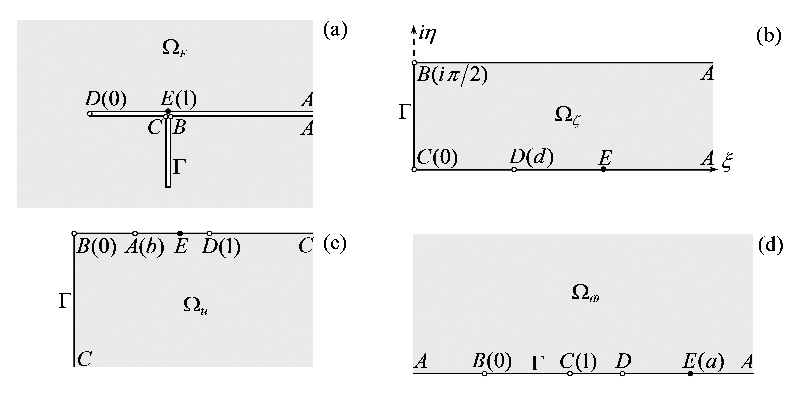
\includegraphics[clip,width=130mm]{Alimov_Fig4.eps}
\caption{Complex planes of the auxiliary variables: (a) $F$; (b) $\zeta = \xi+i\eta$; (c) $u$ and
d) $\omega$.}
 \label{Alimov_Fig4}
\end{figure}

\section{Parametrization and conformal mappings} \label{Alimov:sec5}
The shape of the regions $\Omega_\chi $ and $\Omega_F$ is quite simple. Accordingly, we can hope to
obtain exact formulas for the conformal mapping $\chi \to F$. However, it is difficult to write out
function $F(\chi)$ directly in an explicit form. Similar to many well-known examples from classical
hydrodynamics~\cite{Alimov:bib20}, it is necessary to use some parametrization. By the
parametrization, we mean here the introduction of one or more planes of parametric complex variables
in order to find the parameterized form of the conformal mappings $\chi \to F$, using chains of
well-known conformal mappings. Here it is convenient to introduce one main plane of the parametric
variable $\zeta$ and two auxiliary planes of parametric variables $u$ and $\omega$.

We choose the main plane of the parametric variable $\zeta = \xi + i\eta$ in the form of the
half-strip $\Omega_\zeta $, shown in Fig.~\ref{Alimov_Fig4}~b. The differences between the
half-strip $\Omega_\zeta$ and the half-strip $\Omega_\chi$ are as follows: firstly, the thickness
of $\Omega_\zeta$ is half the thickness of $\Omega_\chi$; and, secondly, infinity in $\Omega_\zeta$
corresponds to the point $A$, while in $\Omega_\chi $ it corresponds to the point $D$, see
Fig.~\ref{Alimov_Fig3}~a and Fig.~\ref{Alimov_Fig4}~b. Note that the position of the boundary point
$D$ in the $\zeta$-plane is specified by an undetermined real parameter $d > 0$.

Further, we choose the auxiliary plane of variable $u$ in the form of the lower right-hand quadrant
$\Omega_u$, shown in Fig.~\ref{Alimov_Fig4}~c. Note that the position of the boundary point $A$ in
the $u$-plane is specified by an undetermined real parameter $b$, which lies in the range $0 < b <
1$.

Furthermore, we choose the auxiliary plane of variable $\omega$ in the form of the upper half-plane
$\Omega_\omega$, shown in Fig.~\ref{Alimov_Fig4}~d. Note that the position of the boundary point $E$
in the $\omega$-plane is specified by an undetermined real parameter $a > 1$.

Let us explain the motivation for the appropriate choice of the shape of the $\zeta$-, $u$-, and
$\omega$-planes. Using the complex $\zeta$-plane allows us to look for the functions $F(\chi)$ and
$W(\chi)$ in a parameterized form, i.e., as a set of three functions $F(\zeta)$, $\chi(\zeta)$ and
$W(\zeta)$. First of all, this $\zeta$-plane must be convenient for finding the meniscus shape.
Well-known examples of solving similar problems in the case of the vertical thin
fiber~\cite{Alimov:bib5}--\cite{Alimov:bib8} shows that our choice of the $\zeta$-plane is
convenient for finding the meniscus shape by integrating the parameterized solution on a
rectangular grid. In addition, the images of the grid points in the physical plane are concentrated
precisely near the fiber, where the meniscus has a complex shape.

The form of the $u$-plane must provide the known conformal mappings $u \leftrightarrows \chi$
(direct and inverse). The form of the $\omega$-plane must provide the known conformal mapping
$\omega \to F$. Moreover, all three planes $\zeta$, $u,$ and $\omega$ must provide the known
conformal mappings $\zeta \rightleftarrows u$, $\zeta \to \omega $ and $u \rightleftarrows \omega$.

Let us write out these known conformal mappings. The quadrant $\Omega_u $ (see
Fig.~\ref{Alimov_Fig4}~c) and the half-strip $\Omega_\chi $ (see Fig.~\ref{Alimov_Fig3}~a) are mapped
conformally onto each other by using the functions~\cite{Alimov:bib13}
\begin{equation}
\label{Alimov:eq47} u(\chi ) = \coth \frac{\chi}{2} \quad \quad \Leftrightarrow \quad \quad \chi
(u) = \ln \left( {\frac{u + 1}{u - 1}} \right).
\end{equation}

The upper half-plane $\Omega_\omega$ (see Fig.~\ref{Alimov_Fig4}~d) is mapped conformally onto the
star-like region $\Omega_F$ (see Fig.~\ref{Alimov_Fig4}~a) by using the function~\cite{Alimov:bib21}
\begin{equation}
\label{Alimov:eq48} F(\omega) = 1 + c(\omega - a)\sqrt {\omega (\omega - 1)},
\end{equation}
where $c$ is an undetermined real parameter.

The quadrant $\Omega_u$ (see Fig.~\ref{Alimov_Fig4}~c) and the half-strip $\Omega_\zeta$ (see
Fig.~\ref{Alimov_Fig4}~b) are mapped conformally onto each other by using the functions similar
to~\eqref{Alimov:eq47}
\begin{equation}
\label{Alimov:eq49} u(\zeta) = b\coth \zeta \quad \quad \Leftrightarrow \quad \quad \zeta (u) =
\frac{1}{2}\ln \left( {\frac{u + b}{u - b}} \right).
\end{equation}

The same half-strip $\Omega_\zeta$ (see Fig.~\ref{Alimov_Fig4}~b) is mapped conformally onto the
upper half-plane $\Omega_\omega$ (see Fig.~\ref{Alimov_Fig4}~d) by using the
function~\cite{Alimov:bib13}
\begin{equation}
\label{Alimov:eq50} \omega (\zeta ) = \cosh ^2\zeta.
\end{equation}

The quadrant $\Omega_u $ (see Fig.~\ref{Alimov_Fig4}~c) and the upper half-plane $\Omega_\omega$ (see
Fig.~\ref{Alimov_Fig4}~d) are mapped conformally onto each other by using the
functions~\cite{Alimov:bib19}
\begin{equation}
\label{Alimov:eq51} u(\omega) = b\sqrt {\frac{\omega}{\omega - 1}} \quad \Leftrightarrow \quad
\omega(u) = \frac{u^2}{u^2 - b^2}.
\end{equation}

Now, using the second expression of~\eqref{Alimov:eq47} and the first expression
of~\eqref{Alimov:eq49}, we can find the exact expression for $\chi(\zeta)$
\begin{equation}
\label{Alimov:eq52} \chi (\zeta) = \ln \left( {\frac{b\coth \zeta + 1}{b\coth \zeta - 1}} \right).
\end{equation}
Using formulas~\eqref{Alimov:eq48} and~\eqref{Alimov:eq50}, we can find the exact expression for
$F(\zeta ):$
\begin{equation}
\label{Alimov:eq53} F(\zeta) = 1 + c\sinh \zeta \cosh \zeta \left( {\cosh^2\zeta - a} \right).
\end{equation}
Knowing functions $\chi (\zeta)$ and $F(\zeta)$, we can also find the function $W(\zeta)$. Indeed,
taking into account~\eqref{Alimov:eq37}, we can write the relation
\begin{equation}
\label{Alimov:eq54} F(\zeta) = \frac{dW}{d\zeta} \left( \frac{d\chi}{d\zeta} \right)^{-1}.
\end{equation}
The derivative ${d\chi / d\zeta}$ can be found by direct differentiation of~\eqref{Alimov:eq52}:
\begin{equation}
\label{Alimov:eq55} \frac{d\chi}{d\zeta} = \frac{2b}{b^2 \cosh^2 \zeta - \sinh^2\zeta } =
\frac{2b}{1 - (1 - b^2) \cosh^2\zeta} .
\end{equation}

If we substitute the formulas~\eqref{Alimov:eq53} and~\eqref{Alimov:eq55} into~\eqref{Alimov:eq54},
we obtain
\begin{equation}
\label{Alimov:eq56} \frac{dW}{d\zeta} = \frac{d\chi}{d\zeta} + 2bc \frac{\sinh \zeta \cosh \zeta
\,(\cosh^2\zeta - a)} {1 - (1 - b^2) \cosh^2\zeta}.
\end{equation}
The right-hand side of this expression can be integrated~\cite{Alimov:bib22}. As a result, we find
the explicit form of the function $W(\zeta)$
\begin{equation}
\label{Alimov:eq57} W(\zeta) = \chi (\zeta) - \frac{bc}{(1 - b^2)}\left\{ {\cosh^2\zeta + \left[
{\frac{1}{(1-b^2)} - a} \right] \ln \left[ {1 - (1-b^2)\cosh^2\zeta} \right]} \right\} - (H_B +
i\pi).
\end{equation}
Here $H_B $ is an integration constant, which is equal to the height of meniscus $Z = H$ at the
point $B$, where $\chi = i\pi$ and $\cosh^2\zeta = \omega = 0$.

Note that the
formulas~\eqref{Alimov:eq47}--\eqref{Alimov:eq49},~\eqref{Alimov:eq51},~\eqref{Alimov:eq52},
and~\eqref{Alimov:eq57} involve the multivalued functions, namely the logarithm and the square root
[19]. Using these functions, we choose their single-valued branches that are real and positive on
the boundary $CD$.

Thus, we have found the exact analytical form of two functions $\chi (\zeta)$ and $W(\zeta)$, which
together represent the desired solution to the problem of the internal asymptotic
expansion~\eqref{Alimov:eq13}--\eqref{Alimov:eq16}. But in the course of its construction we had to
introduce several auxiliary parameters so far undetermined.

\section{Determination of auxiliary parameters} \label{Alimov:sec6}
The direct problem of the inner asymptotic expansion~\eqref{Alimov:eq13}--\eqref{Alimov:eq16}
depends only on the physical parameter $\alpha_0 $ (the angle of fiber inclination), since we fixed
the second physical parameter, namely the contact angle: $\gamma _0 = 0$. However, we have found
not a direct but some parameterized solution of the problem. This solution depends on several
auxiliary parameters, namely $a$, $b$, $c$, $d,$ and $H_B$, which are now to be determined. There
is also parameter $Q$, but we already know its relationship with $\alpha_0$,
see~\eqref{Alimov:eq32}.

In our parameterized solution, we propose to choose the parameter $b$ as the main auxiliary
parameter of the problem, since its relationship with the physical parameter $\alpha_0 $ can be
easily established. Indeed, at the point $A$ we have $u = b$. Taking into account the first
expression of~\eqref{Alimov:eq47}, we can write the identity
\[
A:\quad b = u = \coth \left( {\frac{t_A + i\pi }{2}} \right) = \frac{\sinh t_A}{1 + \cosh t_A}.
\]
Then, using the second expression of~\eqref{Alimov:eq31}, we can establish such a relationship
between $b$ and $\alpha_0 $
\begin{equation}
\label{Alimov:eq58} b = \frac{\cos \alpha_0}{1 + \sin \alpha_0} = \frac{1 - \sin \alpha_0 }{\cos
\alpha_0 }\quad \quad \Leftrightarrow \quad \quad \sin \alpha_0 = \frac{1 - b^2}{1 + b^2},\quad
\cos \alpha_0 = \frac{2b}{1 + b^2}.
\end{equation}
Note that in the limit $\alpha_0 \to 0$ we have $b \to 1$.

All other auxiliary parameters of the problem, namely $a$, $c$, $d,$ and $H_B$, should be expressed
through the main auxiliary parameter $b$.

\subsection{Expression of the parameters $a$, $c$ and $d$ as functions of $b$}
The expression for the parameter $d$ can be found by comparing the position of the point $D$ in the
$\zeta$- and $u$-planes, see Figs.~\ref{Alimov_Fig4}~b and c. Using the second
relation of~\eqref{Alimov:eq49}, we obtain
\begin{equation}
\label{Alimov:eq59} d(b) = \frac{1}{2}\ln \left( {\frac{1 + b}{1 - b}} \right).
\end{equation}

Some relationships between the parameters can be established due to the properties of the conformal
mapping $\omega \to F$ of the star-like region $\Omega_F $ onto the upper half-plane
$\Omega_\omega$~\cite{Alimov:bib21}. Let $\omega_D$ denote the position of the point $D$ in the
$\omega$-plane. The expression $\omega_D $ as a function of $b$ can be obtained by comparing the
position of the point $D$ in the $u$- and $\omega$-planes, see Fig.~\ref{Alimov_Fig4}c and
Fig.~\ref{Alimov_Fig4}d. Using the second relation of~\eqref{Alimov:eq51}, we obtain
\begin{equation}
\label{Alimov:eq60} \omega_D = \left( {1 - b^2} \right)^{-1}.
\end{equation}

At the same time, the parameter $\omega_D$ must satisfy the equation~\cite{Alimov:bib21}
\[
\left. {\frac{1}{\left[ {F(\omega)-1} \right]}\frac{dF}{d\omega}} \right|_{\omega = \omega_D }= 0.
\]
Using the form~\eqref{Alimov:eq48} of the function $F(\omega)$, we arrive at the equation
\[
4\omega_D^2 - 3\omega_D - 2a\omega_D + a = 0.
\]
We can solve this equation for $a$. Then, using~\eqref{Alimov:eq60}, we can obtain the expression
for the parameter $a$:
\begin{equation}
\label{Alimov:eq61} a(b) = \frac{4\omega_D^2 - 3\omega_D}{2\omega_D - 1} = \frac{1+3b^2}{1-b^4}.
\end{equation}

The expression for the parameter $c$ can be found by comparing the position of the point $D$ in the
$F$- and $\omega$-planes, see Figs.~\ref{Alimov_Fig4}~a and d. Using the
form~\eqref{Alimov:eq48} of the function $F(\omega)$, we obtain the equation
\[
1 + c(\omega_D - a)\sqrt {\omega_D (\omega_D - 1)} = 0.
\]
We can solve this equation for $c$. Then, using~\eqref{Alimov:eq60} and~\eqref{Alimov:eq61}, we
obtain the expression $c(b)$:
\begin{equation}
\label{Alimov:eq62} c(b) = \frac{\left( {1 - b^4} \right)\left( {1 - b^2} \right)}{2b^3}.
\end{equation}
Thus, we have found the expressions for the parameters $a$, $c$ and $d$ as functions of $b$. Note
that the form of the function $W(\zeta )$, formula~\eqref{Alimov:eq57}, involves the auxiliary
parameters $a$, $b,$ and $c$. Now we can get rid of the parameters $a$ and $c$. Indeed,
from~\eqref{Alimov:eq61} and~\eqref{Alimov:eq62} we have the following two identities
\[
\frac{bc}{\left( {1 - b^2} \right)} = \frac{1 - b^4}{2b^2}, \quad \quad  \frac{1}{\left( {1 - b^2}
\right)}-a = - \frac{2b^2}{1 - b^4}.
\]
Using these identities, one can significantly simplify the right-hand expression
of~\eqref{Alimov:eq57}
\begin{equation}
\label{Alimov:eq63} W(\zeta) = \chi (\zeta ) - \frac{\left({1 - b^4} \right)}{2b^2}\cosh^2\zeta +
\ln \left[ {1 - \left( {1-b^2} \right)\cosh^2\zeta } \right] - \left( {H_B + i\pi } \right),
\end{equation}
where, instead of the multivalued logarithm function, one should choose such a
single-valued branch that is real and positive at the boundary $CD$. Here the integration constant
$H_B $ also appears. Its definition constitutes the second part of this section.

\subsection{Determination of the integration constant $H_B$}
This constant is involved in the function $H^{(i)}(\xi, \eta) = - \mbox{Re}\, W(\zeta)$. It seems
that the most natural approach to determine the constant $H_B$ is this: we find the value of the
function $H^{(i)}(\xi ,\eta)$ at any of the boundary points $A$, $B$, $C,$ and $D$; then we compare
this value with the known value of the meniscus height $H(X,Y)$ at the same point, provided that
the point lies in the zone $R \sim 1$, where the inner asymptotic expansion is valid. But in this
zone there is not a single point of the boundary with a known meniscus height $H(X,Y)$! The same
can be said about the meniscus height $h(x,y)$ in the $xyz$-coordinate system. The only value of
the function $h(x,y)$ that we know is the value $h = 0$ at infinity $r \to \infty $. But at
infinity the inner asymptotic expansion is not valid!

Therefore, we will have to determine the constant $H_B$, using a rather complicated approach.
Firstly, for this purpose we can use only the condition at infinity~\eqref{Alimov:eq6} of the
original boundary problem~\eqref{Alimov:eq3}--\eqref{Alimov:eq6}. Secondly, since we have made the
transition to the new $XYZ$-coordinate system and to the new function $H(X,Y)$, the
condition~\eqref{Alimov:eq6} for the function $h(x,y)$ should be rewritten as some condition for
the function $H(X,Y)$ at infinity $R \gg 1$. And thirdly, this rewritten
condition~\eqref{Alimov:eq6} can be applied to the function $H^{(i)}(X,Y)$ only indirectly, by
linking $H^{(i)}(X,Y)$ with the function $H^{(u)}(X,Y)$, which uniformly approximates the meniscus
$\Sigma $ everywhere.

Following this scheme, from~\eqref{Alimov:eq6} we obtain that the function $h^{(u)}(x,y)$ must
satisfy the condition $h^{(u)} \to 0$ at infinity $r \to \infty$. In terms of the function
$H^{(u)}(X,Y)$, this leads to the condition
\begin{equation}
\label{Alimov:eq64} R \gg 1: \quad H^{(u)}(X,Y) = X\tan \alpha_0 + o(1),
\end{equation}
 according to formula~\eqref{Alimov:eq10}. Note that on the right-hand side
of~\eqref{Alimov:eq64} the term of order 1, i.e., $O(R^0)$, is equal to zero.

Next, we already have the expression~\eqref{Alimov:eq18}, which links the functions $H^{(i)}(X,Y)$
and $H^{(u)}(X,Y)$. It should be noted that the modified Kelvin function $K_0$ involved in this
expression disappears at infinity~\cite{Alimov:bib14}. Then, we can make sure that
condition~\eqref{Alimov:eq64} for the function $H^{(u)}(X,Y)$ turns into the
condition~\eqref{Alimov:eq16} for the function $H^{(i)}(X,Y)$. As a result, the following
conclusion can be made: in order to determine the constant of integration $H_B$, we can use the
condition at infinity~\eqref{Alimov:eq16} taking into account all terms of order 1, i.e., $O(R^0)$.
A similar conclusion was made in the case of the vertical fiber~\cite{Alimov:bib5}.

Before we apply the condition~\eqref{Alimov:eq16}, it can be simplified as follows: instead of the
neighborhood of infinity in its general form $R \gg 1$, we restrict ourselves to its particular
form $Y = 0$, $X \gg 1$. Using this simplification as well as the formula~\eqref{Alimov:eq32}, we
transform the condition~\eqref{Alimov:eq16} into the following condition
\begin{equation}
\label{Alimov:eq65} Y = 0, \; X \gg 1: \quad  H^{(i)}(X) = X \tan \alpha_0 -
\frac{1}{\cos^2\alpha_0 }\left[ {\ln \left( {\frac{X}{\cos \alpha_0 }} \right) + C_\varepsilon}
\right] + O\left( {X^{-1}\ln X} \right).
\end{equation}
Thus, we have the estimate for the behavior of the boundary function $H^{(i)}(X)$ on $DA$ in the
neighborhood of the point $A$ in the $XY$-plane.

On the other hand, we have the exact expression~\eqref{Alimov:eq63} for the function $W(\zeta)$,
and therefore we can obtain the same exact expressions for the functions $W(\chi)$, $W(u)$, etc.
All these functions will contain the desired constant $H_B$ and consequently any of them can be
used in our analysis. It seems most convenient to use the function $W(u)$. To find its exact form,
we take into account that from the combination of the relation~\eqref{Alimov:eq50} and the second
relation in~\eqref{Alimov:eq51} follows the relation
\[
\cosh^2\zeta = \frac{u^2}{u^2- b^2}.
\]
Substituting this relation as well as the second relation from~\eqref{Alimov:eq47} into the
expression~\eqref{Alimov:eq63}, we obtain such an exact expression for $W(u)$ in the whole
$u$-plane
\begin{equation}
\label{Alimov:eq66} W(u) = \ln \frac{b^2(u + 1)^2}{u^2 - b^2} - \frac{1 - b^4}{2(u^2 - b^2)} -
\left( {H_B + \frac{1 - b^4}{2b^2} + i\pi } \right).
\end{equation}
Taking the real part of~\eqref{Alimov:eq66} and setting $u \in CDA$, we obtain an exact estimate of
the behavior of the boundary function $H^{(i)}(u) = - {\rm Re} W(u)$ on the entire boundary $CDA$
including the neighborhood of the point $A$ in the $u$-plane
\begin{equation}
\label{Alimov:eq67} CDA: \quad H^{(i)}(u) = \ln \frac{u^2 - b^2}{(u + 1)^2} + \frac{1 - b^4}{2(u^2
- b^2)} + \left( {H_B + \frac{1 - b^4}{2b^2} - 2\ln b} \right),\quad \mbox{Im}\, u = 0.
\end{equation}

The desired constant $H_B $ can be determined by equating the estimates~\eqref{Alimov:eq65}
and~\eqref{Alimov:eq67}, obtained for the boundary functions $H^{(i)}(X)$ and $H^{(i)}(u)$ on $DA$
in the neighborhood of point $A$. But for this, we need to additionally use one of the two boundary
functions at least asymptotically in the neighborhood of the point $A$: either $u(X)$ on $DA$ in
the $XY$-plane; or $X(u)$ on $DA$ in the $u$-plane. Accordingly, we can propose \textit{two ways}
for finding the constant $H_B$.

The \textit{first way} is based on the use of the boundary function $u(X)$ on $DA$ in the
$XY$-plane. This function can be estimated using the variable $J$, i.e., the magnitude of the
fictitious flow. Variables $J$ and $t$ are related by the one-to-one
correspondence~\eqref{Alimov:eq22}. Since $t = \mbox{Re}\,\chi$ and the mappings $u
\rightleftarrows \chi$ have already been found, see formula~\eqref{Alimov:eq47}, we can easily
establish the exact expression for the boundary function $u(J)$ on $DA$.

On the other hand, by differentiating the boundary relation~\eqref{Alimov:eq65} with respect to
$X$, we can find ${\partial H^{(i)}}/{\partial X}$ in the neighborhood of infinity $Y = 0$, $X \gg
1$. Accordingly, one can asymptotically estimate $\nabla H^{(i)}$ on $DA$ in the neighborhood of
the point $A$ in the $XY$-plane, since we have ${\partial H^{(i)}}/{\partial Y} = 0$ on $DA$,
see~\eqref{Alimov:eq15}. If we know $\vert \nabla H^{(i)} \vert$, then we can uniquely determine
the magnitude of the fictitious flow $J$, see~\eqref{Alimov:eq20}. Therefore, one can
asymptotically estimate the boundary behavior of the function $J(X)$ on $DA$ in the neighborhood of
the point $A$. Finally, by substituting this estimate into the exact expression for $u(J)$, we can
obtain the desired estimate for the behavior of the boundary function $u(X)$ on $DA$ in the
neighborhood of the point $A$ in the $XY$-plane. So, for example, the integration constant was
found in~\cite{Alimov:bib6}.

However, in our case, the behavior of the boundary function $H^{(i)}(X)$ on $DA$ at infinity,
according to the estimate~\eqref{Alimov:eq65}, is determined not by the singularity $\sim \ln X$,
as in the case of the vertical fiber~\cite{Alimov:bib5},~\cite{Alimov:bib6}, but by the stronger
singularity $\sim X$. Therefore, the terms of the asymptotic expansion~\eqref{Alimov:eq65} of the
function $H^{(i)}(X)$ for small $X^{-1}$ are not sufficient: it is necessary to find higher-order
terms of the expansion~\eqref{Alimov:eq65}. In our case, this seems to be quite a difficult
problem.

The \textit{second way} for finding the constant $H_B $ is based on the use of the boundary
function $X(u)$ on $DA$ in the $u$-plane. This function can be estimated using direct integration
of Khristianovich's differential relations~\eqref{Alimov:eq24}. In general, asymptotic analysis of
such integral for small $X^{-1}$ can also be a difficult problem, but in our case this integral can
be calculated exactly. As a result, it is possible to obtain the exact form of the boundary
function $X(u)$ on the entire boundary $CDA$. The details are given in the \textit{Appendix}, here
we present only the final form of this function
\begin{equation}
\label{Alimov:eq68} CDA: \quad X(u) = 1 - \frac{1 - b^2}{2b}\ln \frac{u - b}{u + b} - \frac{2}{u +
1} + \frac{u(1 + b^2)}{u^2 - b^2}.
\end{equation}
Substituting this formula into the expression~\eqref{Alimov:eq65}, we obtain the first estimate of
the boundary function $H^{(i)}(u)$ on $DA$ in the neighborhood of the point $A$ in the $u$-plane.
The second estimate of this function is given directly by the expression~\eqref{Alimov:eq67}, which
involve $H_B$. Comparing these two estimates, we obtain (see \textit{Appendix})
\begin{equation}
\label{Alimov:eq69} H_B = - \frac{(1 - b)(1 + 3b - b^2 + b^3)}{4b^2} + \frac{1 + b^4}{4b^2}\ln
\frac{8b^2}{(1 + b^2)^2} + \ln \frac{b(1 + b)^2}{\sqrt 2 (1 + b^2)} - \frac{(1 +
b^2)^2}{4b^2}C_\varepsilon,
\end{equation}
where the constant $C_\varepsilon$ is determined by the formula~\eqref{Alimov:eq17}.

\section{Configuration of external menisci} \label{Alimov:sec7}
First, we find the surface $Z = H^{(i)}(X,Y)$, which corresponds to the obtained solution for the
problem of the inner asymptotic expansion (i.e., which approximates the desire meniscus $\Sigma $
only in zone $R \sim 1)$. This solution was parameterized by introducing the auxiliary complex
plane of parametric variable $\zeta = \xi + i\eta $. Accordingly, it is reasonable to look for the
surface $Z = H^{(i)}(X,Y)$ as some parametric surface, i.e., we need to find three functions
$H^{(i)}(\xi, \eta)$, $X(\xi, \eta)$ and $Y(\xi,\eta)$~\cite{Alimov:bib11}.

The first of these functions, namely $H^{(i)}(\xi, \eta)$, can be found by the formula
\begin{equation}
\label{Alimov:eq70} H^{(i)}(\xi, \eta) = - \mbox{Re} \, W(\zeta),
\end{equation}
where the function $W(\zeta)$ is expressed by the exact formulas~\eqref{Alimov:eq63}
and~\eqref{Alimov:eq69}. The remaining functions $X(\xi, \eta)$ and $Y(\xi, \eta)$ can be
determined using the differential relations
\begin{equation}
\label{Alimov:eq71} \frac{\partial }{\partial \xi}\hspace{-0.5mm}\left(
{X\hspace{-1mm}+\hspace{-0.5mm}iY} \right) = e^{i\theta}\hspace{-1.5mm}\left[ {i\cosh t
\frac{\partial \psi}{\partial \xi}}-\sinh t \frac{\partial H^{(i)}}{\partial \xi}
\right]\hspace{-1.0mm}, \;\; \frac{\partial }{\partial \theta}\hspace{-0.5mm}\left(
{X\hspace{-1mm}+\hspace{-0.5mm}iY} \right) = e^{i\theta}\hspace{-1.5mm}\left[ {i\cosh t
\frac{\partial \psi}{\partial \eta}}-\sinh t \frac{\partial H^{(i)}}{\partial
\eta}\right]\hspace{-1.0mm},
\end{equation}
which follow from Khristianovich's formulas~\eqref{Alimov:eq24}. Here the complex
variable $X + iY$ is used only to shorten the expressions (i.e., we do not imply any functions of
the complex variable $X + iY)$.

The partial derivatives appearing in~\eqref{Alimov:eq71} are related to the derivative
${dW}/{d\zeta}$ as follows~\cite{Alimov:bib19}
\[
\frac{dW}{d\zeta} = - \frac{\partial H^{(i)}}{\partial \xi} + i\frac{\partial \psi}{\partial \xi} =
\frac{\partial \psi}{\partial \eta} + i\frac{\partial H^{(i)}}{\partial \eta}.
\]
Then, taking into account the formula~\eqref{Alimov:eq71}, we can obtain the functions $X(\xi,
\eta)$ and $Y(\xi, \eta)$ by using line integrals of vector fields
\begin{equation}
\label{Alimov:eq72}
\begin{array}{c}
 X(\xi, \eta) + iY(\xi, \eta) = 1 + \int\limits_0^\zeta {e^{i\theta}\sinh
t\left[ {\mbox{Re} \left\{ {\frac{dW}{d\zeta }} \right\}d\xi - \mbox{Im}\left\{
{\frac{dW}{d\zeta }} \right\}d\eta } \right]} \\
 + \, i\int\limits_0^\zeta
{e^{i\theta}\cosh t\left[ {\mbox{Im}\left\{ {\frac{dW}{d\zeta }} \right\}d\xi +
\mbox{Re}\left\{ {\frac{dW}{d\zeta}} \right\}d\eta} \right]} ,
 \end{array}
\end{equation}
where the formulas~\eqref{Alimov:eq52} and~\eqref{Alimov:eq56} should be taken into
account. In deriving~\eqref{Alimov:eq72}, we have used that $X_C = 1$ and $Y_C = 0$.

If we use a rectangular grid $\left\{ {\xi_k, \eta_m } \right\}$ in the $\zeta$-plane, then in
formula~\eqref{Alimov:eq72} we can pass from line integrals to ordinary ones, i.e., to integrals
either over $\xi$ or over $\eta$. Indeed, let us introduce into the $\zeta$-plane a rectangular
grid with a uniform step of size $\Delta \xi > 0$ along $\xi$-axis and with a uniform step of size
$\Delta \eta > 0$ along $\eta$-axis:
\[
\xi_k = (k - 1)\Delta \xi, \quad k = 1,...,K; \quad \quad \eta _m = \frac{\pi (m - 1)}{2(M - 1)},
\quad m = 1,...,M.
\]

To ensure good quality of drawing the meniscus in the vicinity of point $D$, the step size $\Delta
\xi$ should be chosen so that the value of parameter $d$, corresponding to this point in the
$\zeta$-plane, coincides with one of the grid point $\xi_{k}'$, see formula~\eqref{Alimov:eq59} and
Fig.~\ref{Alimov_Fig4}~b
\[
D: \quad \eta = 0,\quad \xi_{k}' = d.
\]
Using our rectangular grid, the three functions $H^{(i)}(\xi, \eta)$, $X(\xi, \eta),$ and $Y(\xi,
\eta)$ can be matched to three two-dimensional arrays $H_{km}^{(i)}$, $X_{km}$ and $Y_{km}$. The
two-dimensional array $H_{km}^{(i)}$ corresponding to the function $H^{(i)}(\xi, \eta)$ is
determined by the formula~\eqref{Alimov:eq70}
\begin{equation}
\label{Alimov:eq73} H_{km}^{(i)} = - \mbox{Re} \left. {W(\zeta)} \right|_{\zeta = \xi_k + i\eta_m
}, \quad k = 1,...,K; \quad m = 1,...,M,
\end{equation}
where the formulas~\eqref{Alimov:eq63} and~\eqref{Alimov:eq69} should be used.

The two-dimensional arrays $X_{km}$ and $Y_{km}$ corresponding to functions $X(\xi, \eta)$ and
$Y(\xi, \eta)$ can be found as follows. First, by choosing the contour $\Gamma$: $\xi = 0$, $\eta
\in [0,\pi / 2]$ in the $\zeta$-plane as the integration path in the formula~\eqref{Alimov:eq72},
we can find the shape of this contour in the $XY$-plane
\begin{equation}
\label{Alimov:eq74} \Gamma = BC: \quad \quad X_{1m} + iY_{1m} = 1 +
\hspace{-1mm}\int\limits_0^{\eta_m} {\left. \hspace{-1mm}{e^{i\theta}\hspace{-1mm}\left[ {i\cosh t
\,\mbox{Re} \left\{ {\frac{dW}{d\zeta}} \right\} - \sinh t \,\mbox{Im} \left\{ {\frac{dW}{d\zeta }}
\right\}} \right]} \right|_{\xi = 0} d\eta, }
\end{equation}
where $ m = 1,...,M$. We make sure that the found set of points $(X_{1m},Y_{1m})$
actually forms the unit semicircle $\Gamma = BC$ in the $XY$-plane, see Fig.~\ref{Alimov_Fig2}~b.
Then, we can find the remaining members of the arrays $X_{km}$ and $Y_{km}$ by choosing the straight
lines $\eta = \eta_m $ in the $\zeta$-plane with the origin at the points of the boundary $\Gamma =
BC$ as the integration path in the formula~\eqref{Alimov:eq72}
\begin{equation}
\label{Alimov:eq75} X_{km} + iY_{km} = X_{1m} + iY_{1m} + \hspace{-1mm}\int\limits_0^{\xi_k }
{\left. \hspace{-1mm}{e^{i\theta}\hspace{-1mm}\left[ {\sinh t\,\mbox{Re}\left\{ {\frac{dW}{d\zeta
}} \right\} + i\cosh t\,\mbox{Im}\left\{ {\frac{dW}{d\zeta }} \right\}} \right]} \right|_{\eta =
\eta_m } d\xi},
\end{equation}
where $k = 2,...,K$ and $m = 2,...,M$.

The boundary $CDA$, which corresponds both to the straight line $\eta = 0$ in the $\zeta$-plane and
the index $m = 1$ of the rectangular grid, must be examined separately. On this boundary we have:
the angle $\theta$ is equal to $0$ or $\pi$ by virtue of~\eqref{Alimov:eq34}, and the derivative
${dW}/{d\zeta}$ is real, see Fig.~\ref{Alimov_Fig3}~b and Fig.~\ref{Alimov_Fig4}~b. If we use the
formula~\eqref{Alimov:eq75}, we get
\begin{equation}
\label{Alimov:eq76} CDA: \quad X_{k1} = 1 + \hspace{-1mm}\int\limits_0^{\xi_k } \hspace{-1mm}
{\left. {\cos \theta \sinh t\, \frac{dW}{d\zeta }} \right|_{\eta = 0} d\xi }, \quad \quad Y_{k1} =
0; \quad \quad k = 1,...,K.
\end{equation}

The path of integration in the integral~\eqref{Alimov:eq76} passes through the point $D$: $\xi = d
= \xi_{k}'$, at which $J = 0$ and, therefore, $t \to \infty $, by virtue of~\eqref{Alimov:eq22}.
Thus, the hyperbolic sine involved in the integrand has a singularity at the point $D$: $\sinh t \to
\infty $. Estimates show that the remaining multiplicative part of the integrand at the point $D$
must be equal to zero, and the integrand itself at this point must be integrable. However, applying
standard formulas for numerical integration to the integral~\eqref{Alimov:eq76} leads to large
errors in the vicinity of the point $D$. These difficulties can be avoided by using the exact
expression~\eqref{Alimov:eq68} for the boundary function $X(u)$ on $CDA$. Then, taking into account
the first expression in~\eqref{Alimov:eq49}, instead of the formula~\eqref{Alimov:eq76}, we obtain
the formula
\begin{equation}
\label{Alimov:eq77} CDA: \quad X_{k1} = \left. {X(u)} \right|_{u = b \coth \xi_k }, \quad \quad
Y_{k1} = 0; \quad \quad k = 1,...,K,
\end{equation}
where for $X(u)$ the exact expression~\eqref{Alimov:eq68} should be used.

We have obtained the parametric
equation~\eqref{Alimov:eq73}--\eqref{Alimov:eq75},~\eqref{Alimov:eq77} for the surface $Z =
H^{(i)}(X,Y)$, which approximates the desired meniscus $\Sigma$ in the zone of the inner asymptotic
expansion $R \sim 1$. Now, using the formulas~\eqref{Alimov:eq18} and~\eqref{Alimov:eq32}, we can
find the members of the array $H_{km}^{(u)}$
\begin{equation}
\label{Alimov:eq78} H_{km}^{(u)} =  H_{km}^{(i)} + \frac{1}{\cos^2\alpha_0 }\hspace{-0.5mm}\left[
{K_0\hspace{-1mm}\left( {\varepsilon^{1/2} \sqrt {\frac{X_{km}^2}{\cos^2\alpha_0} + Y_{km}^2}}
\right)\hspace{-1mm} + \frac{1}{2}\ln \left( {\frac{X_{km}^2}{\cos^2\alpha_0} + Y_{km}^2 }
\right)\hspace{-1mm} + C_\varepsilon} \right],
\end{equation}
which corresponds to the function $H^{(u)}(X,Y)$. Expression~\eqref{Alimov:eq78} together
with the formulas~\eqref{Alimov:eq73}--\eqref{Alimov:eq75},~\eqref{Alimov:eq77} represents the
parametric equation of surface $Z = H^{(u)}(X,Y)$, which uniformly approximates the desired
meniscus $\Sigma $ everywhere in the $XY$-plane.

Finally, using the formulas~\eqref{Alimov:eq7} and~\eqref{Alimov:eq8} of the coordinate
transformation $XYZ \to xyz$, we can return to the original Cartesian coordinate system $xyz$:
\begin{equation}
\label{Alimov:eq79} y_{km} = Y_{km}; \quad \quad x_{km} = X_{km} \cos \alpha_0 + H_{km}^{(u)} \sin
\alpha_0; \quad \quad h_{km}^{(u)} = - X_{km} \sin \alpha_0 + H_{km}^{(u)} \cos \alpha_0,
\end{equation}
where $k = 1,...,K$ and $m = 1,...,M$.

The expression~\eqref{Alimov:eq79} together with the
formulas~\eqref{Alimov:eq73}--\eqref{Alimov:eq75},~\eqref{Alimov:eq77} and~\eqref{Alimov:eq78}
represents the parametric equation of the surface $z = h^{(u)}(x,y)$, which uniformly approximates
the desired meniscus $\Sigma $ everywhere in the $xy$-plane.

\section{Analysis of results} \label{Alimov:sec8}
Since we are dealing with an asymptotic formulation of the problem for small Bond number, to
illustrate specific example it is necessary to choose a specific value of this number. We choose
$\varepsilon = 0.01$ so that the error of the uniform asymptotics~\eqref{Alimov:eq79} would be of
the order $0.01$.

Figure~\ref{Alimov_Fig5} shows examples of the configuration of the external meniscus $\Sigma$ for
different values of the inclination angle $\alpha_0 $ of the circular fiber: $a)\, \alpha_0 = 0$,
$b)\, \alpha_0 = \pi/6$, $c)\, \alpha_0 = \pi/4$, and $d)\, \alpha_0 = \pi/3$. The level curves of
constant height $h$ are shown in Fig.~\ref{Alimov_Fig5} as the white lines with an interval of
${\left( {h_{\max} - h_{\min} } \right)}/{23}$, where $h_{\min} = \min [h^{(u)}(x,y)]$ and
$h_{\max} = \max[h^{(u)}(x,y)]$. The contact line $\Gamma_c $ is shown as the black line. In the
case of the vertical fiber ($\alpha_0 = 0)$, the external meniscus $\Sigma$ is characterized by
axial symmetry. At the same time, the inclination of the fiber from the vertical leads to an
asymmetry of $\Sigma$, which increases with increasing angle of fiber inclination from the
vertical.
\begin{figure}%[!tbh]
\renewcommand{\figurename}{Fig.} \centering
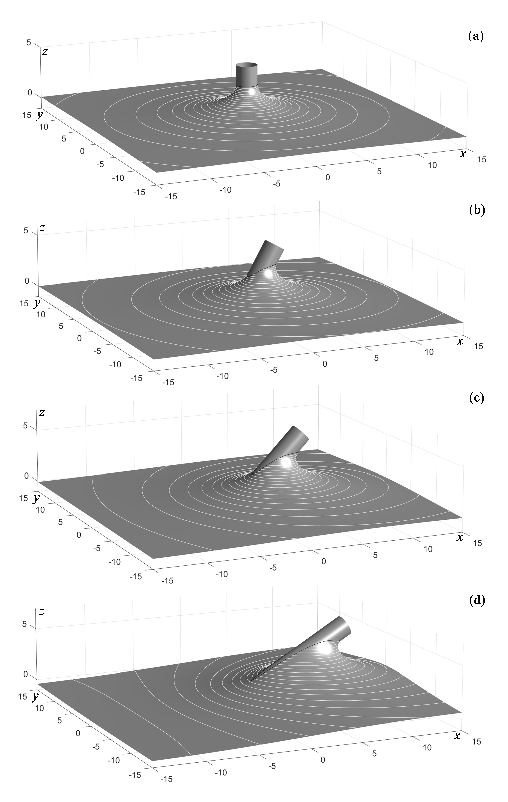
\includegraphics[clip,width=130mm]{Alimov_Fig5.eps}
\caption{Examples of the configuration of the external meniscus $\Sigma$ for $\varepsilon = 0.01$
and for different values of the inclination angle $\alpha_0$ of the circular fiber: a) $\alpha_0 =
0$, b) $\alpha_0 = \pi/6$, c) $\alpha_0 = \pi/4$, d) $\alpha_0 = \pi/3$.}
 \label{Alimov_Fig5}
\end{figure}


As seen in Fig.~\ref{Alimov_Fig5}, when the fiber is tilted to the right, it is the right side of
the contact line $\Gamma_c $ that rises higher than in the case of the vertical fiber. At the same
time, the opposite left side of $\Gamma_c $ falls lower than in the case of the vertical fiber. It
should be noted that such a pattern of meniscus asymmetry differs from our intuitive expectations,
see Fig.~\ref{Alimov_Fig1}~a.

The meniscus asymmetry can be quantitatively assessed by comparing both the heights and the
abscissas of the points $C$ and $B$ depending on the value of $\alpha_0 $, see
Fig.~\ref{Alimov_Fig6}~a, where the solid lines are the graphs $h_C (\alpha_0 )$ and $x_C (\alpha_0
)$; the dashed lines are the graphs $h_B (\alpha_0 )$ and $x_B (\alpha_0 )$.
\begin{figure}%[!tbh]
\renewcommand{\figurename}{Fig.} \centering
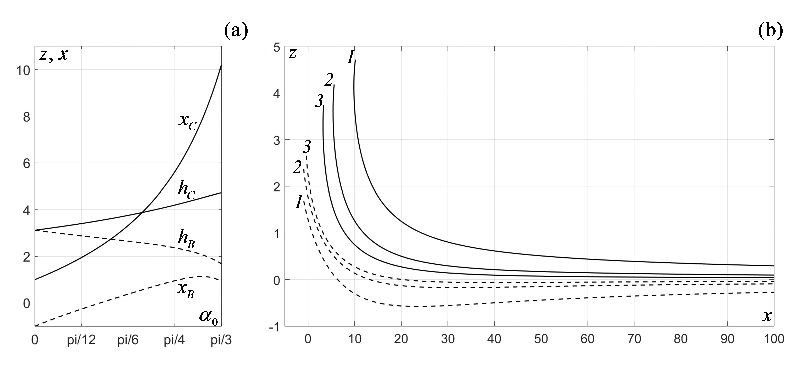
\includegraphics[clip,width=135mm]{Alimov_Fig6.eps}
\caption{(a) Heights $h$ and abscissas $x$ of the points $C$ and $B$ depending on the value of
$\alpha_0$. (b) Graphs $z = h_{CA}(x)$ (solid lines) and $z = h_{BA}(-x)$ (dashed lines) correspond
to the curves $CA$ and $BA$ for $\varepsilon = 0.01$ and for three values of $\alpha_0$: 1 for
$\alpha_0 = \pi/3$, 2 for $\alpha_0 = \pi/4$, 3 for $\alpha_0 = \pi/6$.}
 \label{Alimov_Fig6}
\end{figure}


Note that the lowering of the left side of the contact line $\Gamma_c $ leads to the lowering of
some part of the meniscus $\Sigma$, and this part falls even below than the level $z = 0$ of the
initially undisturbed liquid. This is easy to see in Fig.~\ref{Alimov_Fig5}~d for $\alpha_0 =
\pi/3$, but we maintain that, within the framework of our asymptotic formulation of the problem,
the meniscus always has this qualitative feature for any $\alpha_0 > 0$. For large $\alpha_0 $ the
part of the meniscus, which falls below the level $z = 0$, is located quite close to the fiber; the
magnitude of the smallest lowering of the meniscus $\vert h_{min} \vert$ is quite large; and, hence,
the lowering itself is easy to see. With decreasing $\alpha_0 $, the value of $\vert h_{min} \vert$
decreases rapidly; the part of the meniscus, which falls below the level $z = 0$, moves further and
further away from the fiber; and, hence, it becomes more difficult to see the lowering itself.

To illustrate this effect, in Fig.~\ref{Alimov_Fig6}~b we show the curves $CA$ (solid lines) and
$BA$ (dashed lines) as the cross-sections of the meniscus $\Sigma$ by the vertical $xz$-plane for
three values of $\alpha_0 $: 1 -- $\alpha_0 = \pi/3$, 2 -- $\alpha_0 = \pi/4$, 3 -- $\alpha_0 =
\pi/6$. It is clear that all of these curves tend to zero at infinity, but if on the right side the
curve $CA$ approaches zero from above, then on the left side the curve $BA$ approaches zero from
below!

One more interesting result can be noted: although the highest point of the contact line $\Gamma_c$
lies near the point $C$, it does not coincide with this point itself. This is clearly demonstrated
in Fig.~\ref{Alimov_Fig7}, where for $\alpha_0 = \pi/4$ we present projections of the contact line
$\Gamma_c$: a) onto the $xz$-plane; b) onto the $yz$-plane; and c) onto the $xy$-plane.
\begin{figure}%[!tbh]
\renewcommand{\figurename}{Fig.} \centering
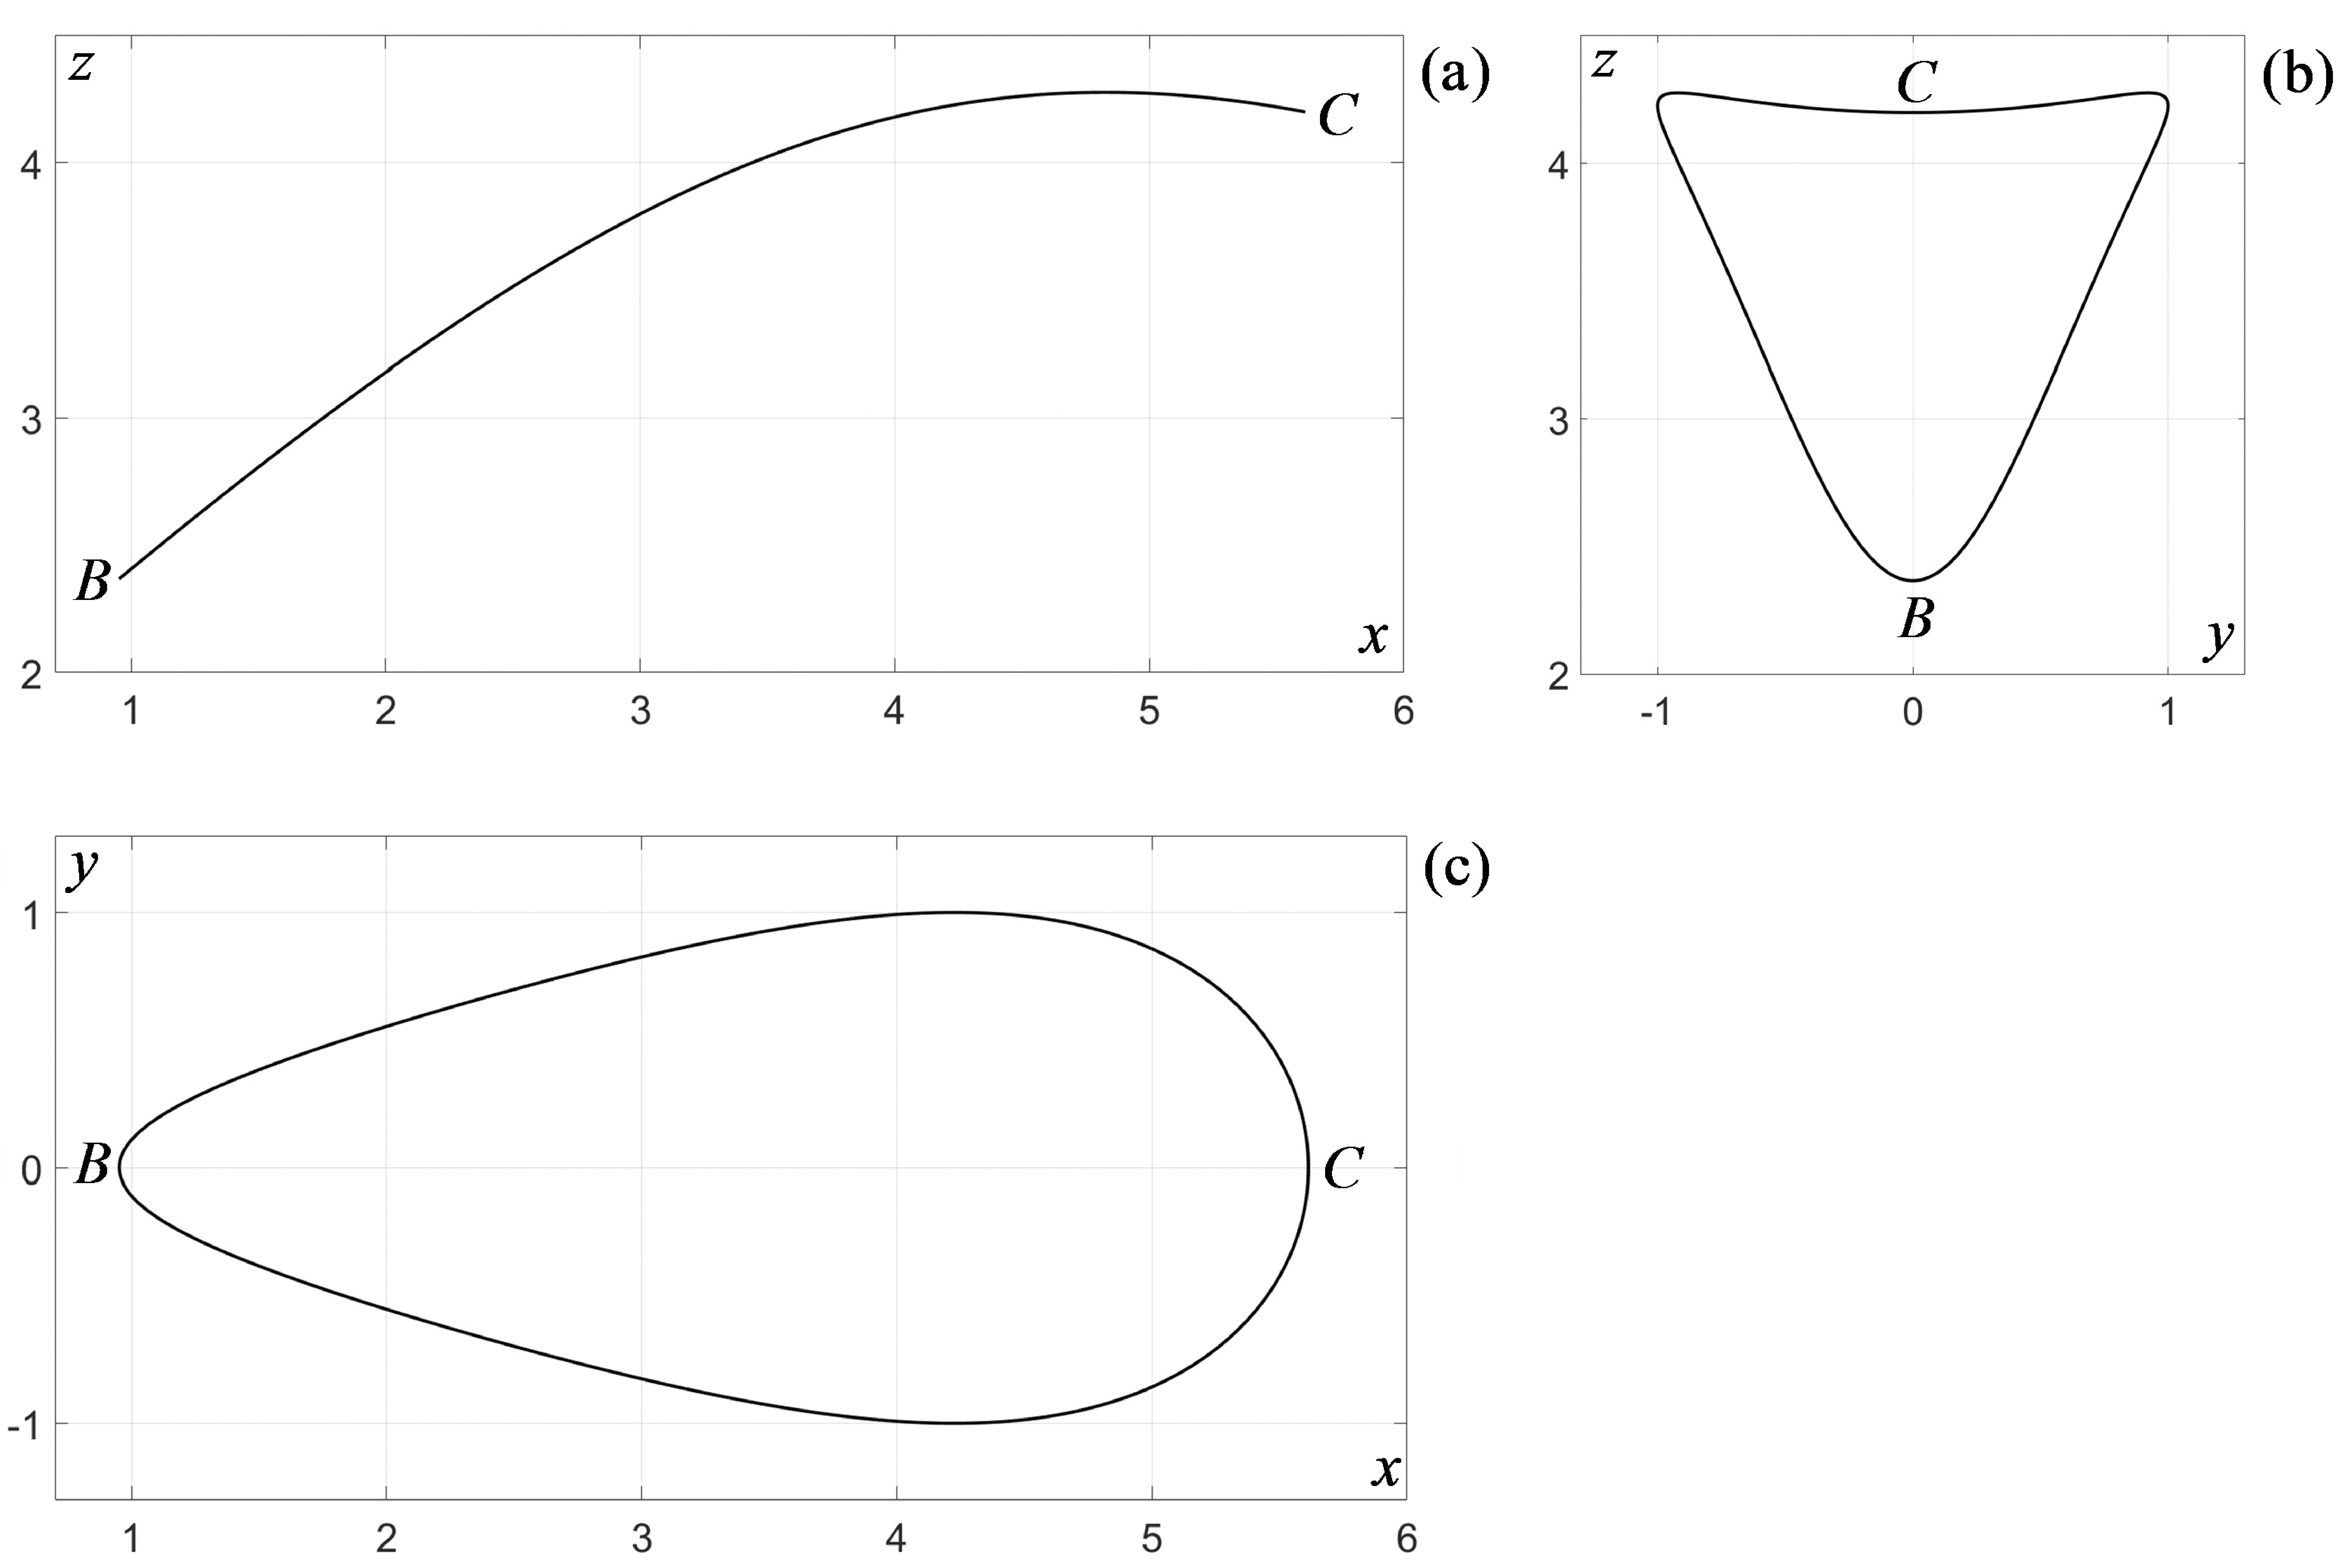
\includegraphics[clip,width=135mm]{Alimov_Fig7.eps}
\caption{Projections of the contact line $\Gamma_c$ for $\varepsilon = 0.01$ and for $\alpha_0 =
\pi/4$: (a) onto the $xz$-plane; (b) onto the $yz$-plane, and (c) onto the $xy$-plane.}
 \label{Alimov_Fig7}
\end{figure}

Note that we limited our analysis of examples to the maximum value of the inclination angle of the
fiber $\alpha _0 = \pi/3$. The exact formulas of the obtained solution allow us to find meniscus
configurations for the inclination angles greater than $\pi/3$, up to $\pi/2$. All noted trends
will manifest themselves even strongly. However, at angles $\alpha_0 > \pi/3$, some doubts arise
about the validity of the asymptotic estimates. Indeed, we estimate the asymptotic parameter
$\varepsilon$ based on the characteristic linear scale $L_m$, which we have chosen to be equal to
half the fiber diameter. But it is more correct to associate the characteristic linear scale not
with the fiber diameter, but with the size of the projection of the contact line $\Gamma_c$ onto
the horizontal $xy$-plane. It is obvious that the maximum size of $\Gamma_c $ in the $y$-direction
is always exactly 2 (fiber diameter). At the same time, the maximum size of $\Gamma_c $ in the
$x$-direction, i.e., value $(x_C - x_B)$, is already approximately 9.3 for $\alpha_0 = \pi/3$, see
Fig.~\ref{Alimov_Fig6}a. This is approximately 4.6 times the fiber diameter, and we believe that
such an increase of the real characteristic scale is already critical. Therefore, the inclination
angles $\alpha_0 > \pi/3$ are not interesting.

Note that the effect of local lowering of the meniscus below level $z = 0$ of the initially
undisturbed liquid for any inclination angle is quite unexpected. It would be interesting to
confirm or disprove this, say, numerically or experimentally.

\section*{CONCLUSIONS}
Using a new asymptotic formulation, we construct an analytical solution for the problem of
determining the configuration of the external meniscus on a thin circular fiber, which is immersed
in a liquid at an arbitrary inclination angle to the vertical, under the assumption that the liquid
completely wets the fiber. It is shown that the contact line becomes asymmetrical: on the side to
which the fiber is inclined, the contact line rises higher, and on the other side it falls lower
than in the case of the vertical fiber. This asymmetry increases with increasing angle of the fiber
inclination to the vertical. Although wetting causes capillary rise of the liquid on the fiber, it
is found that for the inclined fiber some part of the meniscus falls even below the horizontal
level of the initially undisturbed liquid. Within the framework of the accepted asymptotic
formulation of the problem, this effect occurs at any inclination angle different from zero.


\section*{APPENDIX}
% The exact form of the boundary function $X(u)$  on $CDA$ in the $u$-plane. Determination of the integration constant $H_B$}

\textbf{1.} Let us find the exact form of the boundary function $X(u)$ on $CDA$ using
Khristianovich's differential relations~\eqref{Alimov:eq24}. Note that the boundary $CDA$ is a
streamline, and that the angle $\theta$ on $CDA$ is equal to $0$ or $\pi $, see the
conditions~\eqref{Alimov:eq28} and~\eqref{Alimov:eq29}. Then, writing out the first relation
of~\eqref{Alimov:eq24} on this boundary, we obtain
\[
 CDA: \quad dX = - \cos \theta \sinh t \, dH^{(i)} = \sinh \chi \, dW.
\]

The desired boundary function $X(u)$ on $CDA$ can be obtained by integrating this boundary relation
along the boundary itself
\begin{equation}
\label{Alimov:eq80} CDA: \quad X(u) = 1 + \int\limits_\infty^u {\sinh \chi (u)\,\frac{dW}{du}du},
\quad where \; \mbox{Im}\,u = 0.
\end{equation}
Here it is taken into account that $X_C = 1$ and that the variable $u$ on $CDA$ is real,
see Fig.~\ref{Alimov_Fig4}c.

Let's look at the integrand in~\eqref{Alimov:eq80}. The function $\chi(u)$ has already been found,
see the second expression in~\eqref{Alimov:eq47}. Accordingly, we can also find an expression for
$\sinh \chi(u)$
\begin{equation}
\label{Alimov:eq81} \sinh \chi(u) = \frac{1}{2}\left[ {e^{\chi(u)} - e^{-\chi(u)}} \right] =
\frac{1}{2}\left[ {\frac{u + 1}{u - 1} - \frac{u - 1}{u + 1}} \right] = \frac{2u}{(u^2 - 1)}
\end{equation}

The derivative ${dW}/{du}$ can be found by differentiating the expression~\eqref{Alimov:eq66}
\begin{equation}
\label{Alimov:eq82} \frac{dW}{du} = \frac{2}{(u + 1)} - \frac{2u}{u^2 - b^2} + \frac{u(1 -
b^4)}{(u^2 - b^2)^2}.
\end{equation}

We substitute now the expressions~\eqref{Alimov:eq81} and \eqref{Alimov:eq82} into the
formula~\eqref{Alimov:eq80}. As a result, we get
\begin{equation}
\label{Alimov:eq83} CDA: \quad X(u) = 1 - \left. {\mathop {2I(u)}\limits} \right|_\infty ^u ,\quad
where \; \mbox{Im}\,u = 0.
\end{equation}
Here $I(u)$ denotes the integral of a rational function
\begin{equation}
\label{Alimov:eq84} I(u) = - \hspace{-1mm}\int \hspace{-1mm} {\frac{u}{(u^2\hspace{-0.5mm} -
1)}\hspace{-0.5mm}\left[ {\frac{2}{(u + 1)} - \frac{2u}{u^2\hspace{-0.5mm} - b^2} + \frac{u(1 -
b^4)}{(u^2\hspace{-0.5mm} - b^2)^2}}\right]\hspace{-0.5mm}du} = \hspace{-1mm}\int\hspace{-1mm}
{u\frac{2u^2\hspace{-0.5mm} + (1 + b^2)^2u + 2b^4}{(u + 1)^2(u^2\hspace{-0.5mm} - b^2)^2}du}.
\end{equation}
This integral can be calculated exactly in closed form~\cite{Alimov:bib22}. Omitting the details,
we present the final result
\[
 I(u) = \frac{1 - b^2}{4b}\ln \left( {\frac{u - b}{u + b}} \right) + \frac{1}{u + 1} - \left(
\frac{1 + b^2}{2} \right)\frac{u}{u^2 - b^2}.
\]
The validity of this expression can be easily verified by directly differentiating it and by
comparing the result with the formula~\eqref{Alimov:eq84}.

Substituting the found expression for $I(u)$ into the formula~\eqref{Alimov:eq83}, we find the
exact expression for the desired boundary function $X(u)$ on $CDA$
\begin{equation}
\label{Alimov:eq85} CDA: \quad X(u) = 1 - \frac{1 - b^2}{2b}\ln \left( {\frac{u - b}{u + b}}
\right) - \frac{2}{u + 1} + \frac{u(1 + b^2)}{u^2 - b^2}.
\end{equation}
Using this exact expression, in particular, one can obtain an estimate of the boundary function
$X(u)$ on $DA$ in the neighborhood of point $A$ in the $u$-plane. The point $A$ itself in the
$u$-plane corresponds to the value $u = b$, and the neighborhood of this point on the boundary $DA$
corresponds to the interval $0 < u - b < \delta$, where $\delta \ll 1$. Then,
from~\eqref{Alimov:eq85} follows the estimate
\begin{equation}
\label{Alimov:eq86} 0 < u - b < \delta : \quad X(u) = \frac{1 + b^2}{2(u - b)} - \frac{1 -
b^2}{2b}\ln (u - b) + C_X + O(\delta),
\end{equation}
where $C_X $ denotes such a constant
\begin{equation}
\label{Alimov:eq87} C_X = \frac{1 + b^2}{4b} - \frac{1 - b}{1 + b} + \frac{1 - b^2}{2b}\ln (2b).
\end{equation}

\textbf{2.} Let us substitute the found estimate~\eqref{Alimov:eq86} into the
expression~\eqref{Alimov:eq65} for the function $H^{(i)}(X)$. We obtain the following estimate of
the boundary function $H^{(i)}(u)$ on $DA$ in the neighborhood of point $A$ in the $u$-plane
\begin{equation}
\label{Alimov:eq88} H^{(i)}\hspace{-0.5mm}(u) = \frac{(1 + b^2)\tan \alpha_0}{2(u -
b)}\hspace{-0.5mm} + \hspace{-0.5mm}\left[ {\frac{1}{\cos^2\hspace{-0.5mm}\alpha_0} - \frac{\tan
\alpha_0 (1 - b^2)}{2b}} \right]\hspace{-0.5mm}\ln(u - b)\hspace{-0.5mm} + C_H \hspace{-0.5mm}+
O\left( {\delta \ln \delta } \right),
\end{equation}
when $0 < u - b < \delta$.  Here $C_H $ denotes such a constant
\begin{equation}
\label{Alimov:eq89} C_H = C_X \tan \alpha_0 - \frac{1}{\cos^2\alpha_0 }\ln \frac{1 + b^2}{2} +
\frac{1}{\cos^2\alpha_0 }\left( {\ln \cos \alpha_0 - C_\varepsilon } \right).
\end{equation}

Another estimate of this function is given directly by the expression~\eqref{Alimov:eq67}, which
involve the integration constant $H_B$
\begin{equation}
\label{Alimov:eq90} 0 < u - b < \delta : \quad H^{(i)}(u) = \frac{(1 - b^4)}{4b(u - b)} + \ln (u -
b) + \left[ {H_B + \frac{3(1 - b^4)}{8b^2} + \ln \frac{2}{b(1 + b)^2}} \right] + O(\delta).
\end{equation}

The estimates~\eqref{Alimov:eq88} and~\eqref{Alimov:eq90} must coincide. Accordingly, in these
formulas there must equate the terms with singularity $(u - b)^{-1}$, the terms with logarithmic
singularity $\ln (u - b)$ and the terms of order 1. Therefore, we obtain three necessary conditions
\begin{equation}
\label{Alimov:eq91} \frac{(1 + b^2)\tan \alpha_0 }{2} = \frac{(1 - b^4)}{4b},
\end{equation}
\begin{equation}
\label{Alimov:eq92} \frac{1}{\cos^2\alpha_0 } - \frac{\tan \alpha_0 (1 - b^2)}{2b} = 1,
\end{equation}
\begin{equation}
\label{Alimov:eq93} C_X \tan \alpha_0 - \frac{1}{\cos^2\alpha_0 }\ln \frac{1 + b^2}{2} +
\frac{1}{\cos^2\alpha_0 }\left( {\ln \cos \alpha_0 - C_\varepsilon } \right) = H_B + \frac{3(1 -
b^4)}{8b^2} + \ln \frac{2}{b(1 + b)^2},
\end{equation}
where the last condition is obtained by using the formula~\eqref{Alimov:eq89}.

These three conditions involve trigonometric functions of angle $\alpha_0$, which can be expressed
through the main auxiliary parameter $b$ using formula~\eqref{Alimov:eq58}. As a result, we can
verify that the conditions~\eqref{Alimov:eq91} and~\eqref{Alimov:eq92} are satisfied identically
\[
\frac{(1 - b^4)}{4b} \equiv \frac{(1 - b^4)}{4b}, \quad \quad \frac{(1 + b^2)^2}{4b^2} - \frac{(1 -
b^2)^2}{4b^2} \equiv 1.
\]

The last of these three conditions, namely~\eqref{Alimov:eq93}, gives the actual relationship for
determining the integration constant $H_B$. Indeed, taking into account~\eqref{Alimov:eq58}
and~\eqref{Alimov:eq87}, from~\eqref{Alimov:eq93} we obtain
\[
 H_B = - \frac{(1\hspace{-0.5mm} - b)(1\hspace{-0.5mm} + 3b - b^2 + b^3)}{4b^2} +
\frac{1\hspace{-0.5mm} + b^4}{4b^2}\ln \frac{8b^2}{(1\hspace{-0.5mm} + b^2)^2} + \ln
\frac{b(1\hspace{-0.5mm} + b)^2}{\sqrt 2 (1\hspace{-0.5mm} + b^2)} - \frac{(1\hspace{-0.5mm} +
b^2)^2}{4b^2}C_\varepsilon.
\]
\section*{FUNDING}
The author of this work declare that it did not receive financial support.

\section*{CONFLICT OF INTEREST}
The author of this work declare that they have no conflict of interest.


\begin{thebibliography}{25}

\bibitem{Alimov:bib1}
A. W.~Adamson, \textit{Physical Chemistry of Surfaces} (Wiley, New York, 1976).

\bibitem{Alimov:bib2}
D. W.~Langbein, \textit{Capillary surfaces: shape~--~stability~--~dynamics, in particular under
weightlessness} (Springer, New York, 2002).

\bibitem{Alimov:bib3}
L. L.~Lo,  "{The meniscus on a needle -- a lesson in matching}", \ J. Fluid Mech. \textbf{132},
65--78 (1973).

\bibitem{Alimov:bib4}
C.~Pozrikidis, "{Computation of three-dimensional hydrostatic menisci}", \ IMA J. Appl. Math.
\textbf{75}, 418--438 (2010).

\bibitem{Alimov:bib5}
M. M.~Alimov and K. G.~Kornev, "{Meniscus on a shaped fibre: singularities and hodograph
formulation}", \ Proc. R. Soc. A.  \textbf{470}, 20140113 (2014).

\bibitem{Alimov:bib6}
M. M.~Alimov and K. G.~Kornev, "{An external meniscus on a thin ovoidal fiber (the case of full
wetting)}",\  Fluid Dynamics  \textbf{52} (4), 547--560 (2017).

\bibitem{Alimov:bib7}
M. M.~Alimov and K. G.~Kornev, "{External Meniscus on a Ribbon-Like Fiber}", \ Fluid Dynamics
\textbf{53} (Suppl. 1), S40--S58 (2018).

\bibitem{Alimov:bib8}
M. M.~Alimov and K. G.~Kornev, "{An External Meniscus on a Thin Fiber Whose Profile Has Separate
Rectification Points}",\  Russian Mathematics \textbf{64} (1), 3--10 (2020).

\bibitem{Alimov:bib9}
M. M.~Alimov, "{External meniscus on an inclined thin fiber}", \  Russian Mathematics
%\textbf{??} (??), ??-??
(2025).

\bibitem{Alimov:bib10}
R. I.~Nigmatullin, \textit{Dynamics of Multiphase Media} (Hemisphere Publ. Corp., New York, 1990).

\bibitem{Alimov:bib11}
S. P.~Novikov and A. T.~Fomenko,"\textit{Basic Elements of Differential Geometry and Topology}
(Springer, Dordrecht, 1990).

\bibitem{Alimov:bib12}
L. D.~Landau and E. M.~Lifshitz,"\textit{Fluid Mechanics (2nd Ed.)} (Pergamon, 1987; Nauka, Moscow,
1988).

\bibitem{Alimov:bib13}
G. A.~Korn and T. M.~Korn, \textit{Mathematical handbook for scientists and engineers} (McGraw-Hill
Book Company, 1968).

\bibitem{Alimov:bib14}
M.~Abramowitz and I.~Stegun, \textit{Handbook of Mathematical Functions with Formulas, Graphs and
Mathematical Tables}, (DC: National Bureau of Standards, Washington, 1964).

\bibitem{Alimov:bib15}
A. H.~Nayfeh, \textit{Introduction to Perturbation Techniques} (Wiley, New York, 1981).

\bibitem{Alimov:bib16}
M. G.~Bernadiner and V. M.~Entov, \textit{Hydrodynamical Theory for Filtrating Anomalous Liquids},
(Nauka, Moscow, 1975) [in Russian].

\bibitem{Alimov:bib17}
S. A.~Chaplygin, \textit{On Gas jets}, (Gostekhizdat, Moscow, 1949) [in Russian].

\bibitem{Alimov:bib18}
H.~Lamb, \textit{Hydrodynamics} (Cambridge Univ. Press, Cambridge, 1932).

\bibitem{Alimov:bib19}
M. A.~Lavrent'ev and  B. V.~Shabat, \textit{Methods of the theory of functions of complex
variables} (Science, Moscow, 1973) [in Russian].

\bibitem{Alimov:bib20}
M. I.~Gurevich, \textit{Theory of Jets in Ideal Fluids} (Acad. Press, New York, 1965).

\bibitem{Alimov:bib21}
V. I.~Ivanov and V. Yu.~Popov, \textit{Conformal mappings and their applications} (Editorial -- URSS,
Moscow, 2002) [in Russian]

\bibitem{Alimov:bib22}
A. P.~Prudnikov, Yu. A.~Brychkov, and O. I.~Marichev, \textit{Integrals and Series. V. I. Elementary
functions} (Gordon and Breach Science Publishers, 1986).


\end{thebibliography}



\end{document}
